\documentclass[class=math239,notes,tikz]{agony}
\renewcommand{\thechapter}{\Roman{chapter}}
\titleformat{\section}{\pagebreak\normalfont\large\bfseries}{\thesection}{1em}{}
\settowidth{\cftsecnumwidth}{00~}
\renewcommand\cftsecpresnum{}
\setlist[enumerate,1]{label={(\alph*)}}

\title{MATH 239 Fall 2022: Exercises}
\begin{document}
\renewcommand{\contentsname}{MATH 239 Fall 2022:\\{\huge Exercises/Problem Sets}}

\tableofcontents
\pagebreak

\part{Enumeration}

\section{Basic Principles}

\begin{xca}
  Fix integers $n \geq 0$ and $t \geq 1$.
  Consider a randomly chosen multiset of size $n$ with elements of $t$ types.
  For each part below, calculate the probability that the multiset has the stated property,
  and give a brief explanation.
\end{xca}
\begin{enumerate}
  \item Every type of element occurs at most once.
        \begin{sol}
          Every element either appears or not.
          That is, we have $2^t/\binom{n+t-1}{t-1}$
        \end{sol}
  \item Every type of element occurs at least once.
        \begin{sol}
          This is equivalent to including every element,
          then creating a multiset of the remaining $n-t$ spots.
          That gives $\binom{n-1}{t-1}/\binom{n+t-1}{t-1}$.
        \end{sol}
  \item Every type of element occurs an even number of times.
        \begin{sol}
          Make a multiset of size $\frac{n}{2}$ and then double every item:
          $\binom{\frac{n}{2}+t-1}{t-1}/\binom{n+t-1}{t-1}$.
          Note that 0 is even, so we don't require all types appearing.
        \end{sol}
  \item Every type of element occurs an odd number of times.
        \begin{sol}
          Include every element, then create an even multiset
          with the remaining $n-t$ spots:
          $\binom{\frac{n-t}{2}+t-1}{t-1}/\binom{n+t-1}{t-1}$.
        \end{sol}
  \item For $k \in \N$, exactly $k$ types of element occur
        with multiplicity at least one.
        \begin{sol}
          Pick $k$ types, then a multiset of size $n-k$:
          $\binom{t}{k}\binom{n-k+t-1}{t-1}/\binom{n+t-1}{t-1}$.
        \end{sol}
  \item For $k \in \N$, exactly $k$ types of element occur
        with multiplicity at least two.
        \begin{sol}
          Pick $k$ types, then a multiset of size $n-2k$:
          $\binom{t}{k}\binom{n-2k+t-1}{t-1}/\binom{n+t-1}{t-1}$.
        \end{sol}
\end{enumerate}

\begin{xca}
  Consider rolling six fair 6-sided dice, which are distinguishable,
  so that there are $6^6 = 46656$ equally likely outcomes.
  Count how many outcomes are of each of the following types:
\end{xca}
\begin{enumerate}
  \item Six-of-a-kind.
        \boxed{6}
  \item Five-of-a-kind and a single.
        \boxed{(6 \cdot 5) \cdot \binom{6}{1} = 180}
  \item Four-of-a-kind and a pair.
        \boxed{(6 \cdot 5) \cdot \binom{6}{4} = 450}
  \item Four-of-a-kind and two singles.
        \boxed{(6 \cdot 5 \cdot 4) \cdot \frac{\binom{6}{4}\binom{2}{1}}{2} = 1800}
  \item Two triples.
        \boxed{(6 \cdot 5) \cdot \frac{\binom{6}{3}}{2} = 300}
  \item A triple, a pair, and a single.
        \boxed{(6 \cdot 5 \cdot 4) \cdot \binom{6}{3}\binom{3}{2} = 7200}
  \item A triple and three singles.
        \boxed{(6 \cdot 5 \cdot 4 \cdot 3) \cdot \frac{\binom{6}{3}\binom{3}{1}\binom{2}{1}}{3\cdot2} = 7200}
  \item Three pairs.
        \boxed{(6 \cdot 5 \cdot 4) \cdot \frac{\binom{6}{2}\binom{4}{2}}{3\cdot2} = 1800}
  \item Two pairs and two singles.
        \boxed{(6 \cdot 5 \cdot 4 \cdot 3) \cdot \frac{\binom{6}{2}\binom{4}{2}}{2\cdot2} = 16200}
  \item One pair and four singles.
        \boxed{(6 \cdot 5 \cdot 4 \cdot 3 \cdot 2)\cdot\binom{6}{2} = 10800}
  \item Six singles. \boxed{6! = 720}
\end{enumerate}

\begin{xca}
  Let $m \geq 1$, $d \geq 2$, and $k \geq 0$ be integers.
  When rolling $m$ fair dice, each of which has $d$ sides,
  what is the probability of rolling exactly $k$ pairs and $m - 2k$ singles
\end{xca}
\begin{sol}
  There are $k+(m-2k) = m-k$ distinct sides in the roll.
  There are $\frac{d!}{(d-(m-k))!}$ ways to pick those sides.

  Then, there are $\binom{m}{2}\binom{m-2}{2}\cdots\binom{m-2(k-1)}{2} = \prod_{i=0}^{k-1} \binom{m-2i}{2}$
  ways to choose the locations of the pairs.
  Since some of these are duplicates, we divide out $k!$ permutations of pairs.

  Finally, this gives us $\frac{d!}{(d-m+k)!k!}\prod_{i=0}^{k-1}\binom{m-2i}{2}$.
\end{sol}

\begin{xca}\end{xca}
\begin{enumerate}
  \item Prove that $\bijects$ is an equivalence relation.
        \begin{prf}
          We must show reflexivity, symmetry, and transitivity.
          Let $\rl A$, $\rl B$, and $\rl C$ be sets.

          Notice that $\id : \rl A \to \rl A : a \mapsto a$
          is both surjective (there always exists $a$ such that $\id(a) = a$, namely $a$)
          and injective ($\id(a) = \id(b) \implies a = b$).
          Therefore, $\rl A \bijects \rl A$.

          Suppose $\rl A \bijects \rl B$.
          Then, there exists a bijection $f : \rl A \to \rl B$.
          Because $f$ is surjective, a preimage under $f$ exists for all $b \in \rl B$.
          Since $f$ is injective, the preimage of $b$ under $f$ is a single element $a$.

          Define $g : \rl B \to \rl A$ using the unique preimages of $f$.
          This is surjective (for all $a$, there exists $b = f(a)$ such that $g(b) = a$)
          and injective ($g(b) = g(b') \implies f(g(b)) = f(g(b')) \implies b = b'$).
          Then, $g$ is a bijection and $\rl B \bijects \rl A$.

          Suppose $\rl A \bijects \rl B \bijects \rl C$.
          Then, there exist bijections $f : \rl A \to \rl B$ and $g : \rl B \to \rl C$.
          Define $h = g \circ f : \rl A \to \rl C$.
          Then, for all $c \in \rl C$, there exists $a \in \rl A$
          such that $h(a) = g(f(a)) = c$ because of the surjectivity of $g$ and $f$.
          Also, $h(a) = h(a') \implies g(f(a)) = g(f(a')) \implies f(a) = f(a') \implies a = a'$
          by the injectivity of $g$ and $f$, so $h$ is injective.
          Therefore, $h$ is bijective and $\rl A \bijects \rl C$.

          It follows that $\bijects$ is an equivalence relation.
        \end{prf}
  \item Prove Proposition 1.11.
        \begin{prf}
          Suppose $g(f(a)) = a$ and $f(g(b)) = b$ for all $a \in \rl A$ and $b \in \rl B$.

          \WLOG, consider $f : \rl A \to \rl B$.

          Surjectivity: Let $b \in \rl B$.
          Since $f(g(b)) = b$ and $g(b)$ exists, $f$ is surjective.

          Injectivity: Let $a, a' \in \rl A$ and suppose $f(a) = f(a')$.
          Then, $g(f(a)) = g(f(a'))$ which means $a = a'$ by supposition.

          Therefore, $f$ is bijective and likewise for $g$.

          Now, suppose $f(a) = b$. Then, $g(f(a)) = a = g(b)$.
          Likewise if $g(b) = a$, then $f(g(b)) = b = f(a)$.
          Therefore, $f(a) = b \iff g(b) = a$, as desired.
        \end{prf}
\end{enumerate}

\begin{xca}
  Define $f : \Z \to \N$ as follows: for $a \in \Z$,
  $f(a) = \begin{cases}
      2a    & a \geq 0 \\
      -1-2a & a < 0
    \end{cases}$

  Show that $f$ is a bijection by Proposition 1.11.
\end{xca}
\begin{prf}
  We define the function $g : \N \to \Z : b \mapsto \begin{cases}
      \frac{b}{2}    & b \bmod 2 = 0 \\
      -\frac{b+1}{2} & b \bmod 2 = 1
    \end{cases}$

  Then, consider $g(f(a))$.
  If $a \geq 0$, then $g(f(a)) = g(2a) = \frac{2a}{2} = a$ since $2a$ is even.
  Otherwise, $g(f(a)) = g(-(1+2a)) = -\frac{-(2a+1)+1}{2} = a$ since $-(2a+1)$ is odd.

  Now, consider $f(g(b))$.
  If $b = 2k$ is even, then $f(g(2k)) = f(k) = 2k = b$ since $k \geq 0$ (because $b \in \N$).
  Likewise, if $b = 2k+1$ is odd, then $f(g(2k+1)) = f(-(k+1)) = -1-2(-(k+1)) = 2k+2-1 = 2k+1 = b$.

  Therefore, by Proposition 1.11, $f$ is a bijection.
\end{prf}

\begin{xca}
  Complete Example 1.13.
\end{xca}
\begin{prf}
  We must show that $f$ is a bijection from
  the set of subsets of $[n+t-1]$ of size $t-1$
  to set of all multisets of size $n$ with $t$ types $\rl M(n,t)$:
  \begin{quote}
    Given a subset $S \subseteq [n+t-1]$,
    sort it in increasing order $s_1 < \dotsb < s_{t-1}$.
    Then, define $m_i = s_i - s_{i-1} - 1$.
    For convenience, define $s_0 = 0$ and $s_t = n+t$.

    Define $f(S) = (m_1,\dotsc,m_t)$.
  \end{quote}
  The inverse is also given:
  \begin{quote}
    Given a multiset $\mu = (m_1,\dotsc,m_t)$ of size $n$,
    let $s_i = m_1 + \dotsb + m_i + i$.

    Define $f^{-1}(\mu) = \{s_1,\dotsc,s_{t-1}\}$.
  \end{quote}
  Consider $f(f^{-1}(\mu)) = f(f^{-1}(m_1,\dotsc,m_t)) = f(\{s_1,\dotsc,s_{t-1}\})$.
  Notice that the $s_i$ are already in increasing order
  because we add on the $m_i$ terms. Then,
  \begin{align*}
    m'_i & = s_i - s_{i-1} - 1                                                 \\
         & = \qty(\sum_{j=1}^i m_j + i) - \qty(\sum_{j=1}^{i-1} m_j + i-1) - 1 \\
         & = m_i + \sum_{j=1}^{i-1}(m_j - m_j) + (i - i + 1 - 1)               \\
         & = m_i
  \end{align*}
  and we have that $f(f^{-1}(\mu)) = (m'_1,\dotsc,m'_t) = (m_1,\dotsc,m_t) = \mu$.

  Conversely, consider $f^{-1}(f(S)) = f^{-1}(f(\{s_1,\dotsc,s_{t-1}\})) = f^{-1}(m_1,\dotsc,m_t)$.
  \WLOG, suppose that the $s_i$ are already in increasing order. Then,
  \begin{align*}
    s'_i & = i + \sum_{j=1}^i m_j                            \\
         & = \sum_{j=1}^i (m_j + 1)                          \\
         & = \sum_{j=1}^i ((s_j - s_{j-1} - 1) + 1)          \\
         & = (s_1 + \dotsb + s_i) - (s_0 + \dotsb + s_{i-1}) \\
         & = s_i
  \end{align*}
  and it follows that $f^{-1}(f(S)) = \{s'_1,\dotsc,s'_{t-1}\} = \{s_1,\dotsc,s_{t-1}\} = S$.

  Therefore, by Proposition 1.11, $f$ is a bijection, completing Example 1.13.
\end{prf}

\begin{xca}\label{xca:1-7}
  Give bijective proofs of the following identities:
\end{xca}
\begin{enumerate}
  \item For all $n \in \N$, $\sum_{k=0}^n \binom{n}{k}k = n2^{n-1}$
        \begin{prf}
          Consider the set $\rl S$ of subsets of $[n]$ with one ``highlighted'' element.
          For example, $\{1,2,3,\underline{4},10,12\} \subseteq [12]$.

          We can construct $\rl S = \bigcup \rl S_k$
          where $\rl S_k := \{S \in \rl S : \abs{S} = k\}$.
          To construct an element $S$ of $\rl S_k$,
          create a subset of size $k$, of which there are $\binom{n}{k}$,
          then select one of those $k$ elements to highlight.
          This gives $\abs{\rl S_k} = \binom{n}{k}k$.
          As a disjoint union, $\abs{\rl S} = \sum \binom{n}{k}k$.

          Alternatively, construct $S \in \rl S$ directly.
          Pick a single element from $[n]$ to highlight,
          of which there are $n$.
          Then, fill out the rest of the subset using the remaining $n-1$ items,
          of which there are $2^{n-1}$.
          That is, $\abs{\rl S} = n2^{n-1}$.

          Therefore, under the identity bijection,
          $\sum \binom{n}{k}k = \abs{\rl S} = n2^{n-1}$, as desired.
        \end{prf}
  \item For all $n \in \N$, $\sum_{k=0}^n \binom{n}{k}k(k-1) = n(n-1)2^{n-2}$
        \begin{prf}
          Proceed analogously to part (a), but with two highlighted entries in the subset,
          e.g., $\{1,\underline{2},\underline{\overline{4}},6\} \subseteq [10]$.
          Let this set of subsets be $\rl T$.

          As in (a), consider elements of $\rl T_k$.
          We select \emph{two} elements to underline from the $k$ elements in the subset,
          giving us $\binom{n}{k}k(k-1)$.
          Then, as a disjoint union, $\abs{\rl T} = \sum \abs{\rl T_k} = \sum \binom{n}{k}k(k-1)$.

          Again, considering an element of $\rl T$ directly,
          pick two elements to highlight from $n$ and the $n-1$ elements remaining,
          then of the remaining $n-2$ elements construct a subset.
          This gives $\abs{\rl T} = n(n-1)2^{n-2}$.

          Therefore, $\sum \binom{n}{k}k(k-1) = n(n-1)2^{n-2}$, as desired.
        \end{prf}
\end{enumerate}

\begin{xca}
  For an integer $n \geq 1$, give a bijective proof that
  $\sum_{2 \mid n} \binom{n}{k} = \sum_{2 \nmid n} \binom{n}{k}$.
\end{xca}
\begin{prf}
  We must establish a bijection between
  the set of even subsets $\rl E = \{ S \subseteq [n] : 2 \mid \abs{S} \}$
  and the set of odd subsets $\rl O = \{ S \subseteq [n] : 2 \nmid \abs{S} \}$.

  Define $f : S_n \to S_n : f(S) = \begin{cases}
      S \cup \{1\}      & 1 \not\in S \\
      S \setminus \{1\} & 1 \in S
    \end{cases}$

  Let $f_{\rl E}$ and $f_{\rl O}$ be $f$ restricted to the respective set.

  Notice that $f(S)$ always either increases or decreases the size of a set by 1,
  meaning that it will send sets in $\rl E$ to $\rl O$ and vice versa.

  Also, it is obvious that $f(f(S)) = S \cup \{1\} \setminus \{1\}$ or $S \setminus \{1\} \cup \{1\} = S$,
  so $f$ is its own inverse.

  It follows by Proposition 1.11 that $\rl E \bijects \rl O$, as desired.
\end{prf}

\begin{xca}
  Let $n$ be a positive integer.
  Let $\rl S_n$ be the set of ordered pairs of subsets $(A,B)$
  in which $A \subseteq B \subseteq [n]$.
  Let $\rl T_n$ be the set of all functions $f : [n] \to [3]$.
\end{xca}
\begin{enumerate}
  \item What is $\abs{\rl T_n}$?
        \begin{sol}
          Set-theoretically, a function $f : [n] \to [3]$
          is a set of ordered pairs for each value
          $\{(1,f(1)),(2,f(2)),\dotsc,(n,f(n))\}$.
          We pick $n$ values here for $f(1),\dotsc,f(n) \in [3]$.
          That is, $3^n$ choices.
          Therefore, $\abs{\rl T_n} = 3^n$.
        \end{sol}
  \item Define a bijection $g : \rl S_n \to \rl T_n$.
        Explain why $g((A,B)) \in \rl T_n$ for any $(A,B) \in \rl S_n$.
        \begin{sol}
          Given $(A,B) \in \rl S_n$, every element $i \in [n]$ is either:
          (1) not in $A$ or $B$,
          (2) in $B$ but not in $A$, or
          (3) in $A$ (and $B$ since $A \subseteq B$).

          Let $f(i)$ be the number of the case listed above.
          This is a function $[n] \to [3]$, so $f \in \rl T_n$.
        \end{sol}
  \item Define the inverse function $g^{-1} : \rl T_n \to \rl S_n$
        of the bijection $g$ from part (b).
        \begin{sol}
          Construct $A$ and $B$ from $f \in \rl T_n$:

          Read the case list in (b) in reverse. For all $i \in [n]$:
          if $f(i) = 2$, place $i \in B$; if $f(i) = 3$, place $i \in A$.

          Finally, place all elements of $A$ in $B$.
          Then, we have $(A,B) \in \rl S_n$.
        \end{sol}
\end{enumerate}

\begin{xca}
  Fix integers $n \geq 0$ and $k \geq 1$.
  Let $\rl A(n,k)$ be the set of sequences $(a_i) \in \N^k$
  such that $\sum a_i = n$ and $j \mid a_j$ for all $j$.

  Let $\rl B(n,k)$ be the set of sequences $(b_i) \in \N^k$
  such that $\sum b_i = n$ and $b_1 \geq b_2 \geq \dotsb \geq b_k$.

  Construct a pair of mutually inverse bijections
  between the sets $\rl A(n,k)$ and $\rl B(n,k)$.
\end{xca}
\begin{sol}
  \newcommand{\one}{\mathbb{1}}
  Fix $n$ and $k$ and imply the parameters on $\rl A$ and $\rl B$.
  We will treat the sequences as vectors, i.e., $\vb a = (a_1,\dotsc,a_k)$.

  Let $f : \rl A \to \rl B$.
  We will take the sum of vectors of ones.
  Let $\one_i = (\underbrace{1,\dotsc,1}_{\text{$i$ ones}}, \underbrace{0,\dotsc,0}_{\text{$k-i$ zeroes}})$.

  Then, define $f(\vb a) = \sum_{i=1}^k \frac{a_i}{i}\one_i$.
  For example, if $n=7$ and $k=3$,
  \[ f((2,2,3)) = 2(1,0,0) + \frac{2}{2}(1,1,0) + \frac{3}{3}(1,1,1) = (4,2,1) \]
  Notice that since the $\one_i$ are non-increasing for all $i$,
  their linear combination with positive coefficients is also non-increasing.
  Also, we are ``distributing'' the multiples of $i$ into $i$ ones,
  meaning that the sum $\sum a_i = n$ does not change.

  That is, for all $\vb a \in \rl A$, $f(\vb a) = \vb b$ for some $\vb b \in \rl B$.

  We can define an inverse $f^{-1}(\vb b)$ by starting at $i=k$
  and recursively taking out the largest muliple of $i$ from all $k$ entries.

  For the above example, start with $(4,2,1)$ and take out 1 from all 3 entries.
  This sets $a_3 = 1$ and gives $(3,1,0)$.
  Then, take out 1 from the first 2 entries, setting $a_2 = 1$ and giving $(2,0,0)$.
  Finally, take out 2 from the first 1 entry, setting $a_1 = 2$.
  This gives $\vb a = (2,1,1)$, as expected.

  Formally, we define $\vb a = f^{-1}(\vb b)$ as follows:
  \begin{align*}
    a_i'  & = \min\{b_1 - \sum_{j > i} a_i', \dotsc, b_i - \sum_{j > i} a_i'\} \\
    \vb a & = (a_1', 2a_2', \dotsc, ka_k')
  \end{align*}
  which follows the process described above.

  Then, since the processes are inverses, $f$ is a bijection and $\rl A \bijects \rl B$.
\end{sol}

\begin{xca}
  For $n \geq 0$ and $t \geq 2$, prove bijectively that
  $\binom{n+t-1}{t-1} = \sum_{k=0}^n\binom{n-k+t-2}{t-2}$.
\end{xca}
\begin{prf}
  The left-hand side counts the set $\rl S$ of multisets of size $n$ and $t$ types.

  Since there are at least 2 types, partition $\rl S$
  according to the number of times that 1 appears in the multiset.
  Let $\rl S_k = \{ S \in \rl S : \abs{\{1 \in S\}} = k \}$.

  Then, we can ignore the 1's.
  This means to create an element of $\rl S_k$,
  we must create a multiset of size $n-k$ with $t-1$ types
  and then add $k$ 1's.
  This gives us $\abs{\rl S_k} = \binom{(n-k)+(t-1)-1}{(t-1)-1} = \binom{n-k+t-2}{t-2}$.

  Finally, since the number of 1's in a multiset is unique,
  this is a disjoint union and $\abs{\rl S} = \sum \abs{\rl S_k} = \sum \binom{n-k+t-2}{t-2}$.

  Therefore, $\binom{n+t-1}{t-1} = \abs{\rl S} = \sum\binom{n-k+t-2}{t-2}$, as desired.
\end{prf}

\begin{xca}
  For $n \geq 1$ and $t \geq 1$, prove bijectively that
  $\binom{n+t-1}{t-1} = \sum_{k=0}^t\binom{t}{k}\binom{n-1}{k-1}$.
\end{xca}
\begin{prf}
  Again, the LHS counts the set $\rl S$ of multisets of size $n$ and $t$ types.

  Notice that a multiset need not use all $t$ types.
  Consider the set $\rl S_k$ of multisets of size $n$ which use $k \leq t$ types.
  This set will have at least one of each of the $k$ types
  and the remainder is a multiset of $k$ types and size $n-k$.
  That is, there are $\binom{n-k+k-1}{k-1} = \binom{n-1}{k-1}$ of these.
  We also had to pick the $\binom{t}{k}$ types.
  Therefore, $\abs{\rl S_k} = \binom{t}{k}\binom{n-1}{k-1}$.

  Since the number of types used by a multiset is unique,
  this is a disjoint union and $\abs{\rl S} = \sum \abs{\rl S_k} = \sum \binom{t}{k}\binom{n-1}{k-1}$.

  Therefore, $\binom{n+t-1}{t-1} = \abs{\rl S} = \sum\binom{t}{k}\binom{n-1}{k-1}$.
\end{prf}

\begin{xca}
  Choose a permutation $\sigma$ of $\{1, 2, \dotsc, 7\}$ at random,
  so that each of the $7! = 5040$ permutations are equally likely.
  What are the probabilities of the following events?
\end{xca}
\begin{enumerate}[1.]
  \item Numbers 1 and 2 are consecutive
        \begin{sol}
          Let $\sigma_i$ be the index of $i$ in $\sigma$.
          That is, $\sigma_1 = 2$ means 1 is in position 2.

          Consider when 12 appears in the permutation.
          There are 6 choices to place $\sigma_1 = 1,\dotsc,6$
          so that $\sigma_2 = 2,\dotsc,7$.
          There are also 6 choices to place 21.
          Fill the remaining spots with $5!$.
          Therefore, the probability is $\frac{(6+6)5!}{5040} = \frac{2}{7}$.
        \end{sol}
  \item Number 1 is to the left of 2
        \begin{sol}
          There are 7 choices for $\sigma_2$.
          Then, there are $\sigma_2-1$ choices for $\sigma_1$.
          That is, there are $\sum_{\sigma_2=1}^7 (\sigma_2 - 1) = \frac{7\cdot 8}{2} - 7 = 21$
          of these permutations.
          Fill the remaining 5 spots with $5!$.
          Therefore, the probability is $\frac{21\cdot 5!}{5040} = \frac{1}{2}$.
        \end{sol}
  \item No two odd numbers are consecutive
        \begin{sol}
          There are four odd numbers and three evens.
          This means the only way to separate them is to write OEOEOEO.
          We can permute the odd numbers in $4!$ ways and evens in $3!$ ways.
          This gives a probability $\frac{4!\cdot 3!}{5040} = \frac{2}{70}$.
        \end{sol}
\end{enumerate}

\begin{xca}
  Let $r \geq 2$ and $s \geq 2$ be integers.
  Consider a (non-standard) deck of $rs$ cards,
  divided into $s$ suits each with cards of $r$ different values.
  The cards in each suit are numbered $A, 2, 3, \dotsc, r$,
  and $A$ can be either below $2$ or above $r$.
  Choose five cards from such a deck in one of $\binom{rs}{5}$ ways.
  How many ways are there to produce each kind of hand for this
  ``poker in an alternate universe''?
\end{xca}
\begin{enumerate}
  \item Count ``quints'' (five-of-a-kinds).
        \boxed{r}
  \item Count straight flushes.
        \boxed{(r-4)s}
  \item Count quads.
        \boxed{r\binom{s}{4}\cdot\binom{(r-1)s}{1}}
  \item Count full houses.
        \boxed{r\binom{s}{3}\cdot(r-1)\binom{s}{2}}
  \item Count flushes.
        \boxed{s(r! - (r-4))}
  \item Count straights.
        \boxed{(r-4)(5^s - 5)}
  \item Count trips.
        \boxed{r\binom{s}{3}\cdot\qty(s^2\binom{r-1}{2})}
  \item Count two-pairs.
        \boxed{\binom{r}{2}\binom{s}{2}\binom{s}{2}\cdot(s(r-2))}
  \item Count one-pairs.
        \boxed{r\binom{s}{2}\cdot\binom{(r-1)s}{3}}
  \item Count busted hands.
        \boxed{\qty(\binom{r}{5}-(r-4))\cdot(s^5-s)}
\end{enumerate}

\begin{xca}
  The game called ``Crowns and Anchors'' or ``Birdcage''
  was popular on circus midways early in the 20th century.
  It is a game between a Player and the House, played as follows.
  First, the Player wagers $w$ dollars on an integer $p$ from one to six.
  Next, the House rolls three six-sided dice.
  For every die that shows $p$ dots on top, the House pays the Player $w$ dollars,
  but if no dice show $p$ dots on top then the Player's wager is forfeited,
  and goes to the House. (Assume that the dice are fair, so that every outcome is equally likely.)

  For example, if I wager two dollars on the number five,
  and the dice show five, five, and three dots, respectively,
  then the House pays me four dollars for a total of six (a profit of four dollars).
  However, if in this case the dice show four, three, and two dots, respectively,
  then the House takes my wager for a total of zero (a loss of two dollars).
\end{xca}
\begin{enumerate}
  \item For every dollar that the Player wagers,
        how much money should the Player expect to win back in the long run?
        Would you play this game?
        \begin{sol}
          Consider the expected value for each dollar the Player wagers on $k$:

          There are $6^3 = 216$ total outcomes.
          Of these, there is 1 where $k$ appears 3 times,
          5 where $k$ appears twice,
          and $5^2 = 25$ where $k$ appears once.

          This gives an expected value of $\frac{1}{216}(3k + 5(2k) + 25k) = \frac{38}{216}k$.

          The Player will want to maximize payout and always pick $k=6$.

          This gives an expected payout of $\frac{33\cdot6}{216} \approx \$1.06$.
          This is more than the \$1 wager, so the game is worth playing.
        \end{sol}
  \item In a parallel universe there is a game of Crowns and Anchors
        being played with $m \geq 1$ dice, each of which has $d \geq 2$ sides.
        (Assume that the dice are fair, so that every outcome is equally likely.)
        In which universes does the Player win in the long run?
        In which universes does the House win in the long run?
        In which universes is the game completely fair?
        \begin{sol}
          The Player, as above, will always place a dollar on the highest number $d$.

          Then, there are $d^m$ total outcomes.
          For each possible payout $1 \leq i\cdot d \leq m\cdot d$,
          there are $i$ occurrences of $d$
          and there are $(d-1)^{m-i}$ ways to pick the remaining $m-i$ dice.
          As above, we sum to calculate the expected value.

          This gives $\frac{1}{d^m}\sum_{i=1}^m i(d-1)^{m-i}$.
        \end{sol}
\end{enumerate}

\section{Generating Series}

\begin{xca}
  Calculate the following coefficients
\end{xca}
\begin{enumerate}
  \item $[x^8](1-x)^{-7}$
        \begin{sol}
          Apply the Negative Binomial Series to get $\binom{8+7-1}{7-1} = \binom{14}{6} = 3003$
        \end{sol}
  \item $[x^{10}]x^6(1-2x)^{-5}$
        \begin{sol}
          $[x^{10}]x^6(1-2x)^{-5} = [x^4](1-2x)^{-5}$
          where $(1-2x)^{-5} = \sum \binom{n+5-1}{5-1}2^n x^n$ by NBS
          so we have $\binom{4+5-1}{4} 2^4 = 16\binom{8}{4} = 1120$
        \end{sol}
  \item $[x^8](x^3 + 5x^4)(1+3x)^6$
        \begin{sol}
          Expand: $[x^8](x^3 + 5x^4)(1+3x)^6 = [x^8](x^3(1+3x)^6) + [x^8](5x^4(1+3x^6)) = [x^5](1+3x)^6 + 5[x^4](1+3x)^6$.

          Apply the Binomial Theorem: $(1+3x)^6 = \sum \binom{6}{n} 3^n x^n$
          giving $[x^n](1+3x)^6 = 3^n\binom{6}{n}$.

          Finally, $[x^8](x^3 + 5x^4)(1+3x)^6 = 3^6\binom{6}{5} + 5(3^4\binom{6}{4}) = 10449$
        \end{sol}
  \item $[x^9]((1-4x)^5 + (1-3x)^{-2})$
        \begin{sol}
          Expand: $[x^9]((1-4x)^5 + (1-3x)^{-2}) = [x^9](1-4x)^5 + [x^9](1-3x)^{-2}$.

          Apply BT: $(1+(-4x))^5 = \sum_{n=1}^5 \binom{5}{n} (-4)^n x^n$ so $[x^9](1-4x)^5 = 0$.

          Apply NBS: $(1-3x)^{-2} = \sum \binom{n+2-1}{2-1} 3^n x^n$ so $[x^9](1-3x)^{-2} = 3^9\binom{10}{1} = 196830$
        \end{sol}
  \item $[x^n](1-2tx)^{-k}$
        \begin{sol}
          Apply NBS: $(1-2tx)^{-k} = \sum \binom{n+k-1}{k-1} (2t)^n x^n$,
          so we have $\binom{n+k-1}{k-1}(2t)^n$.
        \end{sol}
  \item $[x^{n+1}]x^k(1-4x)^{-2k}$
        \begin{sol}
          Expand: $[x^{n+1}]x^k(1-4x)^{-2k} = [x^{n-k+1}](1-4x)^{-2k}$.

          Apply NBS: $(1-4x)^{-2k} = \sum \binom{n+2k-1}{2k-1} 4^n x^n$.

          This gives $4^{n-k+1}\binom{n-k+1+2k-1}{2k-1} = 4^{n-k+1}\binom{n+k}{2k-1}$.
        \end{sol}
  \item $[x^n]x^k(1-x^2)^{-m}$
        \begin{sol}
          Expand: $[x^n]x^k(1-x^2)^{-m} = [x^{n-k}](1-x^2)^{-m}$.

          Apply NBS: $(1-x^2)^{-m} = \sum \binom{n+m-1}{m-1} x^{2n}$.

          This gives $[x^n]x^k(1-x^2)^{-m} = \begin{cases*}
              \binom{\frac{n}{2}+m-1}{m-1} & $n$ even \\
              0                            & $n$ odd
            \end{cases*}$
        \end{sol}
  \item $[x^n]((1-x^2)^{-k} + (1-7x^3)^{-k})$
        \begin{sol}
          Expand and apply NBS:
          \begin{align*}
             & [x^n]((1-x^2)^{-k} + (1-7x^3)^{-k})                                                                            \\
             & = [x^n](1-x^2)^{-k} + [x^n](1-7x^3)^{-k}                                                                       \\
             & = [x^n]\sum_{m=0}^\infty\binom{m+k-1}{k-1}x^{2m}
            + [x^n]\sum_{m=0}^\infty\binom{m+k-1}{k-1}7^m x^{3m}                                                              \\
             & = \begin{cases}
                   \binom{\frac{n}{2}+k-1}{k-1} & 2 \mid n  \\
                   0                            & 2 \nmid n
                 \end{cases}
            + \begin{cases}
                7^n\binom{\frac{n}{3}+k-1}{k-1} & 3 \mid n  \\
                0                               & 3 \nmid n
              \end{cases}                                                         \\
             & = \begin{cases}
                   \binom{\frac{n}{2}+k-1}{k-1}                                   & 2 \mid n, 3 \nmid n \\
                   7^n\binom{\frac{n}{3}+k-1}{k-1}                                & 2 \nmid n, 3 \mid n \\
                   \binom{\frac{n}{2}+k-1}{k-1} + 7^n\binom{\frac{n}{3}+k-1}{k-1} & 6 \mid n            \\
                   0                                                              & \text{otherwise}
                 \end{cases}
          \end{align*}
          which is a mess.
        \end{sol}
\end{enumerate}

\begin{xca}
  In each case, find an instance of a Binomial Series that begins as shown.
\end{xca}
\begin{enumerate}
  \item $1-2x+3x^2-4x^3+5x^4-6x^5+\dotsb$
        \begin{sol}
          This has coefficients $(-1)^n(n+1) = (-1)^n\binom{n+2-1}{2-1}$
          which comes from the series $(1+x)^{-2}$.
        \end{sol}
  \item $1+3x+6x^2+10x^3+15x^4+21x^5+\dotsb$
        \begin{sol}
          Coefficients are $\binom{2}{2},\binom{3}{2},\binom{4}{2},\dotsc$
          which match $\binom{n+3-1}{3-1}$,
          which comes from the series $(1-x)^{-3}$.
        \end{sol}
  \item $1-x^3+x^6-x^9+x^{12}-x^{15}+\dotsb$
        \begin{sol}
          Consider $x^{3n}$.
          Coefficients $(-1)^n = (-1)^n\binom{n+1-1}{1-1}$ match $(1+x^3)^{-1}$.
        \end{sol}
  \item $1+2x^2+4x^4+8x^6+16x^8+32x^{10}+\dotsb$
        \begin{sol}
          Consider $x^{2n}$.
          Coefficients $2^n$ match $(1-2x^2)^{-1}$.
        \end{sol}
  \item $1-4x^2+12x^4-32x^6+80x^8-192x^{10}+\dotsb$
        \begin{sol}
          Consider $x^{2n}$.
          Divide through $2^n$ to get $(1, -2, 3, -4, 5, -6)$.
          Coefficients $(-1)^n2^n(n+1) = (-2)^n\binom{n+2-1}{2-1}$
          match $(1+2x^2)^{-2}$
        \end{sol}
  \item $1+6x+24x^2+80x^3+240x^4+672x^5+\dotsb$
        \begin{sol}
          Again, divide through by $2^n$ to get $(3,6,10,\dotsc)$
          which we recognize from (b).
          Coefficients $2^n\binom{n+3-1}{3-1}$
          come from $(1-2x)^{-3}$.
        \end{sol}
\end{enumerate}

\begin{xca}
  Give algebraic proofs of these identities from \Cref{xca:1-7}.
\end{xca}
\begin{enumerate}
  \item For all $n \in \N$, $\sum_{k=0}^n\binom{n}{k}k = n2^{n-1}$
        \begin{prf}
          Recall that $\binom{n}{k} = \frac{n!}{k!(n-k)!}$. Then:
          \begin{align*}
            \sum_{k=0}^n\binom{n}{k}k
             & = \sum_{k=0}^n\frac{n!}{k!(n-k)!}k                 \\
             & = \sum_{k=0}^n\frac{n!}{(k-1)!(n-k)!}              \\
             & = n\sum_{k=0}^n\frac{(n-1)!}{(k-1)!((n-1)-(k-1))!} \\
             & = n\sum_{k=-1}^{n-1}\binom{n-1}{k}                 \\
             & = n2^{n-1}
          \end{align*}
          as desired.
        \end{prf}
  \item For all $n \in \N$, $\sum_{k=0}^n\binom{n}{k}k(k-1) = n(n-1)2^{n-2}$
        \begin{prf}
          As in (a) above:
          \begin{align*}
            \sum_{k=0}^n\binom{n}{k}k(k-1)
             & = \sum_{k=0}^n\frac{n!}{(k-2)!(n-k)!}                   \\
             & = n(n-1)\sum_{k=0}^n\frac{(n-2)!}{(k-2)!((n-2)-(k-2))!} \\
             & = n(n-1)\sum_{k=-2}^{n-2}\binom{n-2}{k}                 \\
             & = n(n-1)2^{n-2}
          \end{align*}
          as desired.
        \end{prf}
\end{enumerate}

\begin{xca}
  Calculate $[x^n](1+x)^{-2}(1-2x)^{-2}$.
  Give the simplest expression you can find.
\end{xca}
\begin{sol}
  First, find $A(x) = (1+x)^{-2} = \sum a_n x^n$
  and $B(x) = (1-2x)^{-2} = \sum b_n x^n$:
  \begin{align*}
    (1+x)^{-2}  & = \sum \binom{n+1}{1} (-1)^n x^n = \sum (-1)^n(n+1)x^n \\
    (1-2x)^{-2} & = \sum \binom{n+1}{1} 2^n x^n = \sum 2^n(n+1)x^n
  \end{align*}
  Then, by definition of multiplication of power series,
  \begin{align*}
    [x^n](1+x)^{-2}(1-2x)^{-2} & = [x^n]A(x)B(x)                                       \\
                               & = [x^n]\sum_{n=0}^\infty \sum_{k=0}^n a_k b_{n-k} x^n \\
                               & = \sum_{k=0}^n (-1)^k(k+1) 2^{n-k}(n-k+1)             \\
                               & = 2^n\sum_{k=0}^n \frac{(k+1)(n-k+1)}{(-2)^k}
  \end{align*}
  which does not look like it's getting simpler.
\end{sol}

\begin{xca}\end{xca}
\begin{enumerate}
  \item Let $a \geq 1$ be an integer. For each $n \in \N$,
        extract the coefficient $x^n$ from both sides of this power series identity:
        \[ \frac{(1+x)^a}{(1-x^2)^a} = \frac{1}{(1-x)^a} \]
        to show that $\binom{n+a-1}{a-1} = \sum_{k=0}^{\floor{n/2}}\binom{a}{n-2k}\binom{k+a-1}{a-1}$
        \begin{prf}
          Apply the Binomial Series to get $[x^n]\frac{1}{(1-x)^a} = \binom{n+a-1}{a-1}$.

          For the left-hand side, consider a product $A(x)\cdot B(x) = (1+x)^a \cdot (1-x^2)^{-a}$.

          Then, the Binomial Theorem gives $A(x) = \sum_{n=0}^a \binom{a}{n} x^n$
          and the Binomial Series gives $B(x) = \sum_{n=0}^\infty \binom{n+a-1}{a-1}x^{2n}$.

          After multiplying, we can consider contributions from $B(x)$.
          We can get $x^{2k}$ for $k = 0,\dotsc,\floor{\frac{n}{2}}$
          leaving $x^{n-2k}$ from $A(x)$.

          This gives a coefficient $\sum_{k=0}^{\floor{n/2}}\binom{a}{n-2k}\binom{k+a-1}{a-1}$.

          Therefore, by definition of equality of power series,
          $\binom{n+a-1}{a-1} = \sum_{k=0}^{\floor{n/2}}\binom{a}{n-2k}\binom{k+a-1}{a-1}$,
          as desired.
        \end{prf}
  \item Can you think of a combinatorial proof?
        \begin{prf}
          We are considering the set of multisets of size $n$ and $a$ types.

          In a multiset, every type $t$ can appear either
          an even $m_t = 2k_t$ or odd $m_t = 2k_t+1$ number of times.
          Let $k = \sum k_t$ and partition the set of multisets on $k$.
          Notice that $\sum m_t = (\sum 2k_t) + \abs{\{t : \text{$m_t$ is odd}\}} = n$,
          which means that there are $n-2k$ types appearing an odd number of times.

          Now, we can instead pick a multiset of size $k$ with $a$ types in $\binom{k+a-1}{a-1}$ ways,
          double every entry, and then add the remainders for the $\binom{a}{n-2k}$ odd entries.
          Since $k$ runs from 0 to $\floor{n/2}$ (above gives $\binom{a}{n-2k}=0$),
          $\binom{n+a-1}{a-1} = \sum_{k=0}^{\floor{n/2}}\binom{a}{n-2k}\binom{k+a-1}{a-1}$,
          as desired.
        \end{prf}
\end{enumerate}

\begin{xca}
  Prove the Infinite Sum Lemma.
\end{xca}
\begin{prf}
  Suppose $\rl A_0,\rl A_1,\rl A_2,\dotsc$ are pairwise disjoint sets
  and let $\rl B = \bigcup_{j=0}^\infty \rl A_j$.
  Also, let $\omega : \rl B \to \N$ be a weight function.
  We want to show that $\Phi_{\rl B}^\omega(x) = \sum_{j=0}^\infty \Phi_{\rl A_j}^\omega(x)$.

  Proceed by the definition of equality and addition for power series.

  Let $\Phi_{\rl A_j}(x) = \sum a_{j,n} x^n$ and $\Phi_{\rl B}(x) = \sum b_n x^n$.

  We must show that $b_n = \sum_{j=0}^\infty a_{j,n}$ for all $n \geq 0$.

  Since $\omega$ is a weight function, $\omega^{-1}(n)$ is a finite set.\footnote{Let $\omega^{-1}(n)$ be the preimage of $n$ under $\omega$.}

  Let $m = \max\{j \in \N : \exists k \in \omega^{-1}(n), k \in \rl A_j\}$,
  the minimum $m$ where $\omega^{-1}(n) \subseteq \bigcup_{j=0}^m \rl A_j$.

  Proceed by induction on $m$ to show that $b_n = \sum_{j=0}^m a_{j,n}$.

  If $m = 0$, then $\omega^{-1}(n) \subseteq \rl A_0$ and we just let $b_n = a_{0,n}$.
  If $m = 1$, then $\omega^{-1}(n) \subseteq \rl A_0 \cup \rl A_1$
  and by the ordinary Sum Lemma, $b_n = [x^n]\Phi_{\rl A_0}(x) + [x^n]\Phi_{\rl A_1}(x) = a_{0,n} + a_{1,n}$.

  Otherwise, $m \geq 1$ and we apply the Sum Lemma to $\rl A_m$ and $\bigcup_{j=0}^{m-1}\rl A_{j-1}$
  to get that $b_n = a_{j,n} + \sum_{j=0}^{m-1} a_{j,n} = \sum_{j=0}^m a_{j,n}$, as desired.

  Then, since $\omega^{-1}(n)$ contains no elements in $\rl A_{m+1},\dotsc$
  we know that $a_{m+1,n} = a_{m+2,n} = \dotsb = 0$ and
  we have that $b_n = \sum_{j=0}^m a_{j,n} = \sum_{j=0}^\infty a_{j,n}$.

  Finally, $\Phi_{\rl B}(x) = \sum \Phi_{\rl A_j}(x)$, as desired.
\end{prf}

\begin{xca}\label{xca:genprodlem}
  Extend the Product Lemma to the product of finitely many sets with weight functions.
\end{xca}
\begin{prf}
  Consider finitely many sets $\rl A_1,\dotsc,\rl A_n$ for $n \geq 2$.
  Let $\rl A = \bigcup_{i=1}^n \rl A$.
  Define a weight function $\omega : \rl A \to \N$ a weight function
  which we can restrict to each set $\rl A_i$.
  On the partial unions $\rl B_j = \bigcup_{i=1}^j \rl A_i$,
  define $\sigma_j : \rl B_j \to \N : (a_1,\dotsc,a_j) \mapsto \sum_{i=1}^j \omega(a_i)$.
  Note that $\rl B_n = \rl A$ and write $\sigma = \sigma_n$.

  Proceed to show that $\Phi_{\rl A}^\omega(x) = \prod \Phi_{\rl A_i}^{\omega}(x)$ by induction.

  If $n = 2$, this is the standard Product Lemma and we get that $\sigma_2$ is a weight function
  and $\Phi_{\rl B_2}^{\omega_2}(x) = \prod_{i=1}^2 \Phi_{\rl A_i}^{\omega}(x)$.

  If $n \geq 3$, suppose that $\Phi_{\rl B_{n-1}}^\omega(x) = \prod_{i=1}^{n-1} \Phi_{\rl A_i}^{\omega}(x)$.

  Then, by the Product Lemma, since $\sigma_n(a_1,\dotsc,a_n)
    = \sigma_{n-1}(a_1,\dotsc,a_{n-1}) + \omega(a_n)$,
  we can say that $\sigma_n$ is a weight function and
  $\Phi_{\rl B_{n-1} \times \rl A_n}^{\sigma_n}(x)
    = \Phi_{\rl A}^\sigma(x)
    = \Phi_{\rl A_n}^{\omega}(x) \cdot \prod_{i=1}^{n-1} \Phi_{\rl A_i}^{\omega}(x)
    = \prod_{i=1}^{n} \Phi_{\rl A_i}^{\omega}(x)$
  as desired.

  Therefore, by induction, the Generalized Product Lemma holds.
\end{prf}

\begin{xca}
  Show that for $m,n,k \in \N$,
  $\sum_{j=0}^k(-1)^j\binom{n+j-1}{j}\binom{m}{k-j} = \binom{m-n}{k}$.
\end{xca}
% TODO

\begin{xca}\end{xca}
\begin{enumerate}
  \item Make a list of all the four-letter ``words''
        that can be formed from the ``alphabet'' $\{a, b\}$.
        Define the weight of a word to be the number of occurrences of $ab$ in it.
        Determine how many words there are of weight 0, 1 and 2.
        Determine the generating series.
        \begin{sol}
          There are $2^4 = 16$ possible words.

          There is one word of weight 2, namely $abab$.

          A single occurrence of $ab$ can be placed at the start, middle, or end.
          If at the start/end, there are 3 ways to fill the other 2 letters ($aa$, $bb$, and $ba$).
          Otherwise, there are 4 (since we do not worry about accidentally making another $ab$).
          This gives $3+4+3 = 10$ words of weight 1.

          The remaining 5 words have weight 0. That is, $aaaa$, $bbbb$ and all words beginning with some amount of $b$ followed by $a$ exclusively. 

          This gives a generating series $5 + 10x + 2x^2$.
        \end{sol}
  \item Do the same for five-letter words over the same alphabet, but preferably,
        without listing the words separately.
        \begin{sol}
          There are $2^5 = 32$ possible words.

          Two occurrences can be placed at the start ($ababX$), end ($Xabab$), or split ($abXab$).
          The $X$ can be either $a$ or $b$, giving $3 \times 2 = 6$ words of weight 2.

          A word with no $ab$ in it can only go from a run of $b$'s to $a$'s,
          so if we consider $b^* a^*$ we have 6 words with weight 0.

          This means there are $32 - 6 - 6 = 20$ words with weight 1.

          This gives a genearting series $6 + 20x + 6x^2$.
        \end{sol}
  \item Do the same for six-letter words.
        \begin{sol}
          There are $2^6 = 64$ possible words.

          Three occurrences fit six letters, so there is 1 word of weight 3.

          Two occurrences can be placed in 4 positions:
          $ababXX$, $abXabX$, $abXXab$, $XababX$, $XabXab$, $XXabab$.
          Like in (a), there are 3, 4, 3, 4, 4, and 3 ways to fill the $X$'s.
          This gives $3 + 4 + 3 + 4 + 4 + 3 = 21$ words of weight 2.

          As in (b), there are 7 words with weight 0.

          There remains $64 - 1 - 21 - 7 = 35$ words with weight 1.

          The generating series is therefore $7 + 35x + 21x^2 + x^3$.
        \end{sol}
\end{enumerate}

\begin{xca}\label{xca:2-dice}\end{xca}
\begin{enumerate}
  \item Consider throwing two six-sided dice, one red and one green.
        The weight of a throw is the total number of pips showing on
        the top faces of both dice (that is, the usual score).
        Make a table showing the number of throws of each weight,
        and write down the generating series.
        \begin{sol}
          Construct the table:
          \begin{center}
            \begin{tabular}{c|l|c}
              Sum & Outcomes          & Count \\ \hline
              0   & $\varnothing$     & 0     \\
              1   & $\varnothing$     & 0     \\
              2   & 11                & 1     \\
              3   & 12 21             & 2     \\
              4   & 13 22 31          & 3     \\
              5   & 14 23 32 41       & 4     \\
              6   & 15 24 33 42 51    & 5     \\
              7   & 16 25 34 43 52 61 & 6     \\
              8   & 26 35 44 53 62    & 5     \\
              9   & 36 45 54 63       & 4     \\
              10  & 46 55 64          & 3     \\
              11  & 56 65             & 2     \\
              12  & 66                & 1
            \end{tabular}
          \end{center}
          with generating series $x^2+2x^3+3x^4+4x^5+5x^6+6x^7+5x^8+4x^9+3x^{10}+2x^{11}+x^{12}$.
        \end{sol}
  \item Do the same as for part (a), but throwing three dice:
        one red, one green, and one white
        \begin{sol}
          Construct the table:
          \begin{center}
            \tiny\begin{tabular}{c|l|c}
              Sum & Outcomes                                                                                                    & Count \\ \hline
              0   & $\varnothing$                                                                                               & 0     \\
              1   & $\varnothing$                                                                                               & 0     \\
              2   & $\varnothing$                                                                                               & 0     \\
              3   & 111                                                                                                         & 1     \\
              4   & 112 121 211                                                                                                 & 3     \\
              5   & 113 122 131 212 221 311                                                                                     & 6     \\
              6   & 114 123 132 141 213 222 231 312 321 411                                                                     & 10    \\
              7   & 115 124 133 142 151 214 223 232 241 313 322 331 412 421 511                                                 & 15    \\
              8   & 116 125 134 143 152 161 215 224 233 242 251 314 323 332 341 413 422 431 512 521 611                         & 21    \\
              9   & 126 135 144 153 162 216 225 234 243 252 261 315 324 333 342 351 414 423 432 441 513 522 531 612 621         & 25    \\
              10  & 136 145 154 163 226 235 244 253 262 316 325 334 343 352 361 415 424 433 442 451 514 523 532 541 613 622 631 & 27    \\
              11  & 146 155 164 236 245 254 263 326 335 344 353 362 416 425 434 443 452 461 515 524 533 542 551 614 623 632 641 & 27    \\
              12  & 156 165 246 255 264 336 345 354 363 426 435 444 453 462 516 525 534 543 552 561 615 624 633 642 651         & 25    \\
              13  & 166 256 265 346 355 364 436 445 454 463 526 535 544 553 562 616 625 634 643 652 661                         & 21    \\
              14  & 266 356 365 446 455 464 536 545 554 563 626 635 644 653 662                                                 & 15    \\
              15  & 366 456 465 546 555 564 636 645 654 663                                                                     & 10    \\
              16  & 466 556 565 646 655 664                                                                                     & 6     \\
              17  & 566 656 665                                                                                                 & 3     \\
              18  & 666                                                                                                         & 1
            \end{tabular}
          \end{center}
          which gives generating series $x^3 + 3x^4 + 6x^5 + 10x^6 + 15x^7 + 21x^8 + 25x^9 + 27x^{10} + 27x^{11} + 25x^{12} + 21x^{13} + 15x^{14} + 10x^{15} + 6x^{16} + 3x^{17} + x^{18}$.
        \end{sol}
\end{enumerate}

\begin{xca}
  Construct a table, as in Exercise 2.10(a),
  if the weight of a throw is defined to be
  the absolute value of the difference between
  the number of pips showing on the two dice.
  Also, write down the generating series.
\end{xca}
\begin{sol}
  Construct the table:
  \begin{center}
    \begin{tabular}{c|l|c}
      Sum & Outcomes                      & Count \\ \hline
      0   & 11 22 33 44 55 66             & 6     \\
      1   & 12 21 23 32 34 43 45 54 56 65 & 10    \\
      2   & 13 24 31 35 42 46 53 64       & 8     \\
      3   & 14 25 36 41 52 63             & 6     \\
      4   & 15 26 51 62                   & 4     \\
      5   & 16 61                         & 2
    \end{tabular}
  \end{center}
  giving generating series $6 + 10x + 8x^2 + 6x^3 + 4x^4 + 2x^5$.
\end{sol}

\begin{xca}
  Let $\rl S$ be the set of ordered pairs $(a, b)$ of integers with $0 \leq \abs{b} \leq a$.
  Each part gives a function $\omega$ defined on the set $\rl S$.
  Determine whether or not $\omega$ is a weight function on the set $\rl S$.
  If it is not, then explain why not.
  If it is a weight function, then determine
  the generating series $\Phi_{\rl S}(x)$ of $\rl S$ with respect to $\omega$,
  and write it as a polynomial or a quotient of polynomials.
\end{xca}
\begin{enumerate}
  \item For $(a,b) \in \rl S$, let $\omega((a,b)) = a$.
        \begin{sol}
          This is a weight function. First, $a \geq 0$ for all $(a,b)$.

          Given finite $a \in \Z$ with $a \geq \abs{b} \geq 0$,
          there are finitely many $b$ to choose from, namely, $-a \leq b \leq a$.
          That is, there are $2a+1$ options for $(a,b)$ given $\omega((a,b)) = a$.

          Therefore, $\Phi_{\rl S}(x) = \sum (2n+1) x^n = 2x\sum n x^{n-1} + \sum x^n
            = \frac{2x}{(1-x)^2} + \frac{1}{1-x} = \frac{1+x}{(1-x)^2}$.
        \end{sol}
  \item For $(a,b) \in \rl S$, let $\omega((a,b)) = a+b$.
        \begin{sol}
          This is not a weight function.
          Notice that $\omega^{-1}(0)$ has infinite size,
          namely, given any $a \geq 0$, set $b = a$ so that $\omega((a,b)) = 0$.
        \end{sol}
  \item For $(a,b) \in \rl S$, let $\omega((a,b)) = 2a+b$.
        \begin{sol}
          This is a weight function. First, $a \geq \abs{b} \geq 0$ means $2a+b \geq 0$.

          Given $\omega((a,b)) = n$, we can construct $n$ as $2a + b$
          for $a = \ceil{\frac{n}{3}},\dotsc,n$
          and corresponding $b = n-2a = n-2\ceil{\frac{n}{3}},\dotsc,-n$.
          That is, $\omega^{-1}(n)$ has size $n-\ceil{\frac{n}{3}}+1$.

          This means $\Phi_{\rl S}(x) = \sum(n-\ceil{\frac{n}{3}}+1)x^n
            = \sum n x^n - \sum\ceil{\frac{n}{3}}x^n + \sum x^n$.
          Write
          \begin{align*}
            \sum\ceil*{\frac{n}{3}}x^n
             & = x + x^2 + x^3 + 2x^4 + 2x^5 + 2x^6 + \dotsb                            \\
             & = (x + 2x^4 + \dotsb) + (x^2 + 2x^5 + \dotsb) + (x^3 + 2x^6 + \dotsb)    \\
             & = x(1 + 2x^3 + \dotsb) + x^2(1 + 2x^3 + \dotsb) + x^3(1 + 2x^3 + \dotsb) \\
             & = (x+x^2+x^3)\sum(n+1)x^{3n}                                             \\
             & = \frac{x+x^2+x^3}{(1-x^3)^2}
          \end{align*}

          By part (a), we know the other series give $\frac{x}{(1-x)^2} - \frac{x+x^2+x^3}{(1-x^3)^2} + \frac{1}{1-x}$.
        \end{sol}
\end{enumerate}

\begin{xca}
  Let $\rl S = [6]^4$ be the set of outcomes when rolling four six-sided dice.
  For $(a,b,c,d) \in S$, define its weight to be $\omega(a,b,c,d) = a+b+c+d$.
  Consider the generating series $\Phi_{\rl S}(x)$ of $\rl S$ with respect to $\omega$.
\end{xca}
\begin{enumerate}
  \item Explain why $\Phi_{\rl S}(x) = \qty(\frac{x-x^7}{1-x})^4$.
        \begin{sol}
          The inner term gives the finite geometric series for $1+x+x^2+x^3+x^4+x^5+x^6$.
          This is exactly $\Phi_{[6]}(x)$.
          By the Generalized Product Lemma (\Cref{xca:genprodlem}),
          the generating series for $\rl S = [6]^4$ is $(\Phi_{[6]}(x))^4$.
        \end{sol}
  \item How many outcomes in $\rl S$ have weight 19?
        % TODO
  \item Let $m$, $d$, $k$ be positive integers.
        When rolling $m$ dice, each of which has exactly $d$ sides,
        how many different ways are there to roll
        a total of $k$ pips on the top faces of the dice?
        \begin{sol}
          The general generating series is $\Phi(x) = \qty(\frac{x-x^{d+1}}{1-x})^m$.
          We want $[x^k]\Phi(x)$.
          % TODO
        \end{sol}
\end{enumerate}

\begin{xca}
  Let $\rl A$ be a set with weight function $\omega : \rl A \to \N$.
  Show that for any $n \in \N$, the number of $\alpha \in \rl A$
  with $\omega(\alpha) \leq n$ is $[x^n]\frac{1}{1-x}\Phi_{\rl A}(x)$.
\end{xca}
\begin{prf}
  By the Binomial Series, $B(x) = \frac{1}{1-x} = 1+x+x^2+\dotsb$, i.e., $b_n = 1$ for all $n$.

  When we multiply $\Phi_{\rl A}(x) = \sum a_n x^n$ by $\frac{1}{1-x}$,
  the product coefficient is by definition $\sum_{i=0}^n a_i b_{n-i} = \sum_{i=0}^n a_i$.
  That is, the sum of the $a_i$ for $i \leq n$.

  But since $a_i$ is the number of elements of $\alpha \in \rl A$ with $\omega(\alpha) = i$,
  we have counted the number of elements $\omega(\alpha) \leq n$.
\end{prf}

\begin{xca}\label{xca:2-15}
  For each of the following sets of compositions,
  obtain a rational function formula for the generating series of that set
  with respect to size.
\end{xca}
\begin{enumerate}
  \item Let $\rl A$ be the set of compositions of length congruent to 1 (modulo 3).
        \begin{sol}
          The allowed sizes for a part are $P = \{1,\dotsc,\}$
          so $\Phi_P(x) = \frac{x}{1-x}$.

          We can generate compositions of length $3k+1$ as $P(P^3)^k$.
          In general, $\rl A = P(P^3)^*$.

          Then, by the Product Lemma, the generating series for $P^3$ is $(\frac{x}{1-x})^3$
          and by the String Lemma, the generating series for $(P^3)^*$ is
          $\sum (\frac{x}{1-x})^{3j} = \frac{1}{1-x^3/(1-x)^3} = \frac{(1-x)^3}{(1-x)^3-x^3}$.

          Finally, $\Phi_{\rl A}(x) = \frac{x(1-x)^3}{(1-x)(1-3x+3x^2-2x^3)}
            = \frac{x-2x^2+x^3}{1-3x+3x^2-2x^3}$.
        \end{sol}
  \item Let $\rl B$ be the set of compositions of length congruent to 2 (modulo 3).
        \begin{sol}
          Proceed as in (a) up to the last multiplication, then square $\Phi_P$ to get
          $\Phi_{\rl B}(x) = \frac{x^2(1-x)^3}{(1-x)^2(1-3x+3x^2-2x^3)}
            = \frac{x^2 - x^3}{1-3x+3x^2-2x^3}$.
        \end{sol}
  \item Let $\rl C$ be the set of compositions of even length,
        with each part being at most 3.
        \begin{sol}
          Here, $P = \{1,2,3\}$, so $\Phi_P(x) = x+x^2+x^3$.

          Then, to get even length, $\rl C = (P^2)^*$.

          By the Product Lemma, $\Phi_{P^2}(x) = (x+x^2+x^3)^2$
          and by the String Lemma, we have
          $\Phi_{\rl C}(x) = \frac{1}{1-(x+x^2+x^3)^2}
            = \frac{1}{1-x^2-2x^3-3x^4-2x^5-x^6}$.
        \end{sol}
  \item Let $\rl D$ be the set of compositions of odd length,
        with each part being at least 2.
        \begin{sol}
          Let $P = \{2,3,\dotsc\}$ so $\Phi_P(x) = x^2 + x^3 + \dotsb
            = x^2(1 + x + \dotsb) = \frac{x^2}{1-x}$.

          Then, to get odd length, $\rl D = P(P^2)^*$.
          By the Product Lemma, $\Phi_{P^2} = \frac{x^4}{(1-x)^2}$
          and by the String Lemma $\Phi_{(P^2)^*} = \frac{1}{1-x^4(1-x)^{-2}}
            = \frac{(1-x)^2}{(1-x)^2-x^4} = \frac{1-2x+x^2}{1-2x+x^2-x^4}$.

          Finally, by the Product Lemma, $\Phi_{\rl D} = \frac{x^2-2x^3+x^4}{(1-x)(1-2x+x^2-x^4)}
            = \frac{x^2-2x^3+x^4}{1-3x+3x^2-x^3-x^4+x^5}$
        \end{sol}
  \item Let $\rl E$ be the set of compositions $\gamma = (c_i)$ of any length,
        in which each part $c_i$ is congruent to $i$ (modulo 2).
        So $c_1$ is odd, $c_2$ is even, $c_3$ is odd, and so on.
        \begin{sol}
          If $\rl O = \{1,3,5,\dotsc\}$ and $\rl P = \{2,4,6,\dotsc\}$,
          we can write $\rl E = (\rl O\rl P)^* \cup (\rl O\rl P)^*\rl O
            = (\rl O\rl P)^*(\{\varepsilon\} \cup \rl O)$
          depending on if the length is even or odd.

          Write $\Phi_{\rl O} = x + x^3 + \dotsb = x(1 + x^2 + \dotsb) = \frac{x}{1-x^2}$
          and $\Phi_{\rl P} = x^2(1 + x^2 + \dotsb) = \frac{x^2}{1-x^2}$.

          Then, by the Product Lemma, $\Phi_{\rl{OP}} = \frac{x^3}{(1-x^2)^2}$
          and by the String Lemma, $\Phi_{(\rl{OP})^*} = \frac{1}{1-x^3(1-x^2)^{-2}}
            = \frac{(1-x^2)^2}{(1-x^2)^2-x^3}$.

          Finally, by the Product and Sum Lemmas,
          $\Phi_{\rl E} = \frac{(1-x^2)^2}{(1-x^2)^2-x^3}\qty(1+\frac{x}{1-x^2})
            = \frac{(1-x^2)^2}{(1-x^2)^2-x^3}\cdot\frac{1+x-x^2}{1-x^2}
            = \frac{(1-x^2)(1+x-x^2)}{(1-x^2)^2-x^3}
            = \frac{1+x-2x^2-x^3+x^4}{1-2x^2-x^3+x^4}$.
        \end{sol}
\end{enumerate}

\section{Binary Strings}

\begin{xca}
  Prove Lemma 3.9 (Unambiguous Expressions)
\end{xca}
\begin{prf}
  Let $\rx R$ and $\rx S$ be regular expressions producing $\rl R$ and $\rl S$.
  Proceed by cases.

  If $\rx R = \varepsilon$, 0, or 1, then $\rl R = \{\varepsilon\}$, $\{0\}$, or $\{1\}$.
  Notice each is produced exactly once, so $\rx R$ is unambiguous.

  Now, suppose $\rx R$ and $\rx S$ are unambiguous.
  We proceed by contrapositives.

  Suppose $\rx R \smile \rx S$ which produces $\rl R \cup \rl S$ is ambiguous.
  Then, since $\rx R$ and $\rx S$ are unambiguous,
  the union operation must produce a duplicate.
  That is, $\rl R \cap \rl S \neq \varnothing$.
  Conversely, if $\rl R \cap \rl S$ is non-empty,
  then whatever expressions are in the intersection are produced twice by $\rx R \smile \rx S$.
  Therefore, $\rx R \smile \rx S$ is ambiguous if and only if $\rl R \cap \rl S \neq \varnothing$.

  Suppose $\rx R\rx S$ is ambiguous.
  Then, $\rl R \rl S = \{\rho\sigma : \rho \in \rl R, \sigma \in \rl S\}$
  produces some element $\rho\sigma = \rho'\sigma'$ twice.
  Notice that for all $(\rho,\sigma) \in \rl R \times \rl S$, $f(\rho,\sigma) = \rho\sigma \in \rl R \rl S$.
  That is, $\abs{\rl R \times \rl S} \geq \abs{\rl R \rl S}$.
  However, since $\rho\sigma = \rho'\sigma'$, $f$ is not injective.
  Therefore, $\abs{\rl R \times \rl S} \neq \abs{\rl R \rl S}$.
  This means $\rl R\times\rl S \mathrel{\not\bijects} \rl R\rl S$.

  Conversely, suppose $\rl R\times\rl S \mathrel{\not\bijects} \rl R\rl S$.
  Then, $\abs{\rl R \times \rl S} > \abs{\rl R \rl S}$.
  This means that under $f$, multiple pairs must be sent to one string,
  which is exactly what it means for $\rl R\rl S$ to be ambiguous.

  Finally, consider $\rx R^*$ is ambiguous.
  Then, since $\rx R$ is unambiguous, the ambiguity must be introduced
  by either a single $\rx R^k$ being ambiguous or the union.
  By induction on the second point, the union is unambiguous if and only if
  $\bigcup_{k=0}^\infty \rl R^k$ is a disjoint union.
  Therefore, $\rx R^*$ is ambiguous if and only if all the $\rx R^k$ are unambiguous
  and the union of the $\rl R^k$ is disjoint.
\end{prf}

\begin{xca}
  Let $\rx A = (10 \smile 101)$ and $\rx B = (001 \smile 100 \smile 1001)$.
  For each of $\rx{AB}$ and $\rx{BA}$, is the expression unambiguous?
  What is the generating series (by length) of the set it produces?
\end{xca}
\begin{sol}
  Write out $\rl{AB} = \{10001, 10100, 101001, 101001, 101100, 1011001\}$.
  Notice $101001$ appears twice, so $\rx{AB}$ is ambiguous.
  The (meaningless) generating series is $2x^5 + 2x^6 + x^7$.

  Write out $\rl{BA} = \{00110, 001101, 10010, 100101, 100110, 1001101\}$.
  No element appeared twice, so $\rx{BA}$ is unambiguous.
  The generating series is $2x^5 + 3x^6 + x^7$.
\end{sol}

\begin{xca}
  Let $\rx A = (00 \smile 101 \smile 11)$ and $\rx B = (00 \smile 001 \smile 10 \smile 110)$.
  Prove that $\rx A^*$ is unambiguous and $\rx B^*$ is ambiguous.
  Find the generating series (by length) for the set $\rl A^*$ produced by $\rx A^*$.
\end{xca}
\begin{sol}
  Notice that $\rx A$ is unambiguous.
  There is no way to combine any two of the three strings to create the other one:
  creating 00 from 101 and 11 is clearly impossible;
  11 from 00 and 101 can only be made by 101101 but 10 and 01 cannot be made by 00;
  101 cannot be made from 00 and 11 since there is no single 0.
  Therefore, $\rx A^*$ is unambiguous.

  For $\rx B$, notice that $00110 = (001)(10) = (00)(110)$, so it is ambiguous.

  By Theorem 3.13, $\Phi_{\rl A^*} = (A^*)(x) = \frac{1}{1-A(x)} = \frac{1}{1-2x^2-x^3}$.
\end{sol}

\begin{xca}
  For each of the following sets of binary strings,
  write an unambiguous expression which produces that set.
\end{xca}
\begin{enumerate}
  \item Binary strings that have no block of 0's of size 3,
        and no block of 1's of size 2.
        \begin{sol}
          A valid block of 0's is matched by $0 \smile 00 \smile 00000^*$.
          Likewise, a valid block of 1's is $1 \smile 1111^*$.
          Then, the block decomposition is
          \[
            \rx R = (\varepsilon \smile 0 \smile 0^2 \smile 0^40^*)
            ((1\smile 1^31^*)(0 \smile 0^2 \smile 0^40^*))^*
            (\varepsilon \smile 1 \smile 1^31^*)
          \]
          which is, as a block decomposition, unambiguous.
        \end{sol}
  \item Binary strings that have no substring of 0's of length 3,
        and no substring of 1's of length 2.
        \begin{sol}
          This means blocks of 0's have length 1 or 2, i.e., $(0 \smile 00)$
          and blocks of 1's have length 1, i.e., $(1)$.
          Then, the block decomposition is
          \[
            \rx R = (\varepsilon \smile 0 \smile 00)(1(0 \smile 00))^*(\varepsilon \smile 1)
          \]
          which an unambiguous block decomposition.
        \end{sol}
  \item Binary strings in which the substring 011 does not occur.
        \begin{sol}
          There are no ways that 011 overlaps itself.
          Therefore, we need only force blocks of 1's after a 0 to have length 1.
          Using a block decomposition depending if we start with 1 or 0,
          \[
            \rx R = \varepsilon \smile (1 1^*)(0 0^* 1)^*0^* \smile (00^*)(1 00^*)^*(\varepsilon \smile 1)
          \]
          which is unambiguous.
        \end{sol}
  \item Binary strings in which the blocks of 0's have even length and
        the blocks of 1's have odd length.
        \begin{sol}
          Blocks of 0's are matched by $00(00)^*$ and 1's by $1(11)^*$. Then,
          \[
            (00)^*(1(11)^*00(00)^*)^*(\varepsilon \smile 1(11)^*)
          \]
          is an unambiguous block decomposition.
        \end{sol}
\end{enumerate}

\begin{xca}
  Let $\rx G = 0^*((11)^*1(00)^*00 \smile (11)^*11(00)^*0)^*$,
  and let $\rl G$ be the set of binary strings produced by $\rx G$.
\end{xca}
\begin{enumerate}
  \item Give a verbal description of the strings in the set $\rl G$.
        \begin{sol}
          The set of binary strings where blocks of 0's
          have the opposite parity of the preceding block of 1's.
        \end{sol}
  \item Find the generating series (by length) of $\rl G$.
        \begin{sol}
          We know by Theorem 3.13 $\Phi_{\rl G}(x) = G(x)$, so
          \begin{align*}
            \Phi_{\rl G}(x)
             & = \frac{1}{1-x}\cdot\frac{1}{1-\qty(\frac{x}{1-x^2}\cdot\frac{x^2}{1-x^2} + \frac{x^2}{1-x^2}\cdot\frac{x}{1-x^2})} \\
             & = \frac{1}{1-x}\cdot\frac{1}{1-\frac{2x^3}{(1-x^2)^2}}                                                              \\
             & = \frac{1}{1-x}\cdot\frac{(1-x^2)^2}{(1-x^2)^2-2x^3}                                                                \\
             & = \frac{(1+x)(1-x^2)}{1-2x^2-2x^3+x^4}                                                                              \\
             & = \frac{1+x-x^2-x^3}{1-2x^2-2x^3+x^4}
          \end{align*}
          as desired.
        \end{sol}
  \item For $n \in \N$, let $g_n$ be the number of strings in $\rl G$ of length $n$.
        Give a recurrence relation and enough initial conditions
        to uniquely determine $g_n$ for all $n \in \N$.
        \begin{sol}
          Apply Theorem 4.8 and read off the linear recurrence relation:
          \[
            g_n - 2g_{n-2} - 2g_{n-3} + g_{n-4} = \begin{cases}
              1  & n = 0    \\
              1  & n = 1    \\
              -1 & n = 2    \\
              -1 & n = 3    \\
              0  & n \geq 4
            \end{cases}
          \]
          from which we calculate initial conditions $g_0 = 1$,
          $g_1 = 1$, $g_2 = 2g_0 - 1 = 1$, $g_3 = 2g_1 + 2g_0 - 1 = 3$.
        \end{sol}
\end{enumerate}

\begin{xca}\end{xca}
\begin{enumerate}
  \item Show that the generating series (by length) for binary strings
        in which every block of 0's has length at least 2
        and every block of 1's has length at least 3 is $\frac{(1-x+x^3)(1-x+x^2)}{1-2x+x^2-x^5}$.
        \begin{sol}
          This set of strings is produced by
          $\rx R = (\varepsilon \smile 000^*)(1111^*000^*)^*(\varepsilon \smile 1111^*)$.
          This leads to the rational function
          \begin{align*}
            R(x)
             & = \qty(1 + \frac{x^2}{1-x})\frac{1}{1-(\frac{x^3}{1-x}\cdot\frac{x^2}{1-x})}\qty(1 + \frac{x^3}{1-x}) \\
             & = \frac{1-x+x^2}{1-x}\cdot\frac{1}{1-\frac{x^5}{(1-x)^2}}\cdot\frac{1-x+x^3}{1-x}                     \\
             & = \frac{(1-x+x^2)(1-x+x^3)}{(1-x)^2}\cdot\frac{(1-x)^2}{(1-x)^2-x^5}                                  \\
             & = \frac{(1-x+x^2)(1-x+x^3)}{1-2x+x^2-x^5}
          \end{align*}
          which is equal to the generating series by Theorem 3.13.
        \end{sol}
  \item Give a recurrence relation and enough initial conditions to
        determine the coefficients of this power series.
        \begin{sol}
          Expand the numerator to get $\Phi_{\rl R}(x) = \frac{1-2x+2x^2-x^4+x^5}{1-2x+x^2-x^5}$.
          Then, apply Theorem 4.8 to read off the linear recurrence relation:
          \[
            r_n - 2r_{n-1} + r_{n-2} - r_{n-5} = \begin{cases}
              1  & n = 0    \\
              -2 & n = 1    \\
              2  & n = 2    \\
              0  & n = 3    \\
              -1 & n = 4    \\
              1  & n = 5    \\
              0  & n \geq 6
            \end{cases}
          \]
          and calculate $r_0 = 1$, $r_1 = -2 + 2r_0 = 0$,
          $r_2 = 2 + 2r_1 - r_0 = 1$, $r_3 = 0 + 2r_2 - r_1 = 2$,
          $r_4 = -1 + 2r_3 - r_2 = 2$, and $r_5 = 1 + 2r_4 - r_3 + r_0 = 4$.
        \end{sol}
\end{enumerate}

\begin{xca}\end{xca}
\begin{enumerate}
  \item For $n \in \N$, let $h_n$ be the number of binary strings of length $n$
        such that each even-length block of 0's is followed by a block of exactly one 1
        and each odd-length block of 0's is followed by a block of exactly two 1's.
        Show that $h_n = [x^n]\frac{1+x}{1-x^2-2x^3}$.
        \begin{sol}
          Let $\rl H$ be the relevant set and notice it is produced by
          the block decomposition $\rx H = 1^*(00(00)^*1 \smile 0(00)^*11)$.
          Note that since a block of 0's is followed by a block of 1's, we must end on a block of 1's.
          By Theorem 3.11, $\Phi_{\rl H}(x) = H(x)$ which is
          \begin{align*}
            H(x)
             & = \frac{1}{1-x}\cdot\frac{1}{1-(\frac{x^3}{1-x^2} + \frac{x^3}{1-x^2})} \\
             & = \frac{1}{1-x}\cdot\frac{1-x^2}{1-x^2-2x^3}                            \\
             & = \frac{1+x}{1-x^2-2x^3}
          \end{align*}
          and $h_n = [x^n]H(x)$ by Proposition 2.7, as desired.
        \end{sol}
  \item Give a recurrence relation and enough initial conditions to
        determine $h_n$ for all $n \in \N$.
        \begin{sol}
          Again, read off a recurrence relation from $H(x)$ by Theorem 4.8:
          \[
            h_n - h_{n-2} - 2h_{n-3} = \begin{cases}
              1 & n = 0    \\
              1 & n = 1    \\
              0 & n \geq 2
            \end{cases}
          \]
          and calculate $h_0 = 1$, $h_1 = 1$, $h_2 = 0 + h_0 = 1$,
          and $h_3 = 0 + h_1 + 2h_0 = 3$.
        \end{sol}
\end{enumerate}

\begin{xca}
  Let $\rl K$ be the set of binary strings in which any block of 1's
  which immediately follows a block of 0's must have length at least
  as great as the length of that block of 0's.
\end{xca}
\begin{enumerate}
  \item Derive a formula for $K(x) = \sum_{\kappa \in \rl K} x^{\ell(\kappa)}$.
        \begin{sol}
          First, we recursively define $\rx L = 11^* \smile 0\rx L 1$
          so that $\rl L = 0^i 1^j$ where $j \geq i \geq 1$ which is unambiguous.
          Now, define $\rx K = 1^*\rx L^* 0^*$ as a block decomposition.

          We can now calculate $L(x) = \frac{x}{1-x} + x^2L(x)$
          so $L(x) = \frac{x}{(1-x)(1-x^2)}$. Then,
          \begin{align*}
            K(x)
             & = \frac{1}{1-x}\cdot\frac{1}{1-\frac{x}{(1-x)(1-x^2)}}\cdot\frac{1}{1-x} \\
             & = \frac{1}{(1-x)^2}\cdot\frac{(1-x)(1-x^2)}{(1-x)(1-x^2)-x}              \\
             & = \frac{1+x}{1-2x-x^2+x^3}
          \end{align*}
          which is the generating series $\Phi_{\rl K}(x)$ by Theorem 3.11.
        \end{sol}
  \item Give a recurrence relation and enough initial conditions to
        determine the coefficients $[x^n]K(x)$ for all $n \in \N$.
        \begin{sol}
          Let $k_n = [x^n]K(x)$. By Theorem 4.8, we have the recurrence relation
          \[
            k_n - 2k_{n-1} - k_{n-2} + k_{n-3} = \begin{cases}
              1 & n = 0    \\
              1 & n = 1    \\
              0 & n \geq 2
            \end{cases}
          \]
          and calculate $k_0 = 1$, $k_1 = 1 + 2k_0 = 3$,
          and $k_2 = 0 + 2k_1 + k_0 = 7$.
        \end{sol}
\end{enumerate}

\begin{xca}\end{xca}
\begin{enumerate}
  \item Fix an integer $m \geq 1$.
        Find the generating series (by length) of the set of binary strings
        in which no block has length greater than $m$.
        \begin{sol}
          Blocks of 0's and 1's become $\smilesum_{i=1}^m 0^i$
          and $\smilesum_{i=1}^m 1^i$.
          Then, the block decomposition
          \[
            \rx R = (\smilesum_{i=0}^m 0^i)
            (\smilesum_{i=1}^m 1^i\smilesum_{i=1}^m 0^i)^*
            (\smilesum_{i=0}^m 1^i)
          \]
          produces our desired set.
          By Theorem 3.11, the generating series $\Phi_{\rl R}(x) = R(x)$ which is
          \begin{align*}
            R(x)
             & = \qty(\sum_{i=0}^m x^i)\qty(\frac{1}{1-(\sum_{i=1}^m x^i)^2})\qty(\sum_{i=0}^m x^i) \\
             & = \qty(\frac{1-x^{m+1}}{1-x})^2\qty(\frac{1}{1-(\frac{x-x^{m+1}}{1-x})^2})           \\
             & = \frac{(1-x^{m+1})^2}{(1-x)^2}\cdot\frac{(1-x)^2}{(1-x)^2-(x-x^{m+1})^2}            \\
             & = \frac{(1-x^{m+1})^2}{(1-x)^2-(x-x^{m+1})^2}
          \end{align*}
          which I'm sure simplifies further.
        \end{sol}
  \item Fix integers $m, k \geq 1$.
        Find the generating series (by length) of the set of binary strings
        in which no block of 0's has length greater than $m$
        and no block of 1's has length greater than $k$.
        \begin{sol}
          Proceed as above: we instead get the block decomposition
          \[
            \rx R = (\smilesum_{i=0}^m 0^i)
            (\smilesum_{i=1}^k 1^i\smilesum_{i=1}^m 0^i)^*
            (\smilesum_{i=0}^k 1^i)
          \]
          which produces the set we want. By Theorem 3.11,
          \begin{align*}
            \Phi_{\rl R}(x)
             & = R(x)                                                                                                                   \\
             & = \qty(\sum_{i=0}^m x^i)\qty(\frac{1}{1-(\sum_{i=1}^k x^i)(\sum_{i=1}^m x^i)})\qty(\sum_{i=0}^k x^i)                     \\
             & = \qty(\frac{1-x^{m+1}}{1-x})\qty(\frac{1}{1-(\frac{x-x^{k+1}}{1-x})(\frac{x-x^{m+1}}{1-x})})\qty(\frac{1-x^{k+1}}{1-x}) \\
             & = \frac{(1-x^{m+1})(1-x^{k+1})}{(1-x)^2}\cdot\frac{(1-x)^2}{(1-x)^2 - (x-x^{k+1})(x-x^{m+1})}                            \\
             & = \frac{(1-x^{m+1})(1-x^{k+1})}{(1-x)^2 - (x-x^{k+1})(x-x^{m+1})}                                                        \\
          \end{align*}
          as desired.
        \end{sol}
\end{enumerate}

\begin{xca}
  Let $\rl L$ be the set of binary strings in which
  each block of 1's has odd length, and which do not contain the substring 0001.
  Let $\rl L_n$ be the set of strings in $\rl L$ of length $n$
  and let $L(x) = \sum_{n=0}^\infty \abs{\rl L_n}x^n$.
\end{xca}
\begin{enumerate}
  \item Give an expression that produces the set $\rl L$ unambiguously,
        and explain briefly why it is unambiguous and produces $\rl L$.
        \begin{sol}
          Notice that 0001 does not overlap itself.
          Then, we need only prevent a non-terminal block of 3 or more 0's.
          Also, blocks of 1's must be odd.
          Write $\rx L = (\varepsilon \smile 1(11)^*)((0 \smile 00)1(11)^*)^*0^*$
          and notice it is unambiguous as a block decomposition.
        \end{sol}
  \item Use your expression from part (a) to show that
        $L(x) = \frac{1+x-x^2}{1-x-x^2+x^3+x^4}$.
        \begin{sol}
          By Theorem 3.11, the generating series $L(x)$ is
          \begin{align*}
            L(x)
             & = (1+\frac{x}{1-x^2})\frac{1}{1-\frac{(x+x^2)x}{1-x^2}}\frac{1}{1-x} \\
             & = \frac{1+x-x^2}{(1-x^2)(1-x)}\cdot\frac{1-x^2}{1-x^2-(x+x^2)x}      \\
             & = \frac{1+x-x^2}{(1-x)(1-2x^2-x^3)}                                  \\
             & = \frac{1+x-x^2}{1-x-x^2+x^3+x^4}
          \end{align*}
          as desired.
        \end{sol}
\end{enumerate}

\begin{xca}
  Let $\rl M$ be the set of binary strings in which
  each block of 0's has length at most two
  and which do not contain 00111 as a substring.
  Let $\rl M_n$ be the set of strings in $\rl M$ of length $n$
  and let $M(x) = \sum_{n=0}^\infty \abs{\rl M_n}x^n$.
\end{xca}
\begin{enumerate}
  \item Give an expression that produces the set $\rl M$ unambiguously,
        and explain briefly why it is unambiguous and produces $\rl M$.
        \begin{sol}
          Write $\rx M = 1^*(011^* \smile (001 \smile 0011))^*(\varepsilon \smile 0 \smile 00)$.
          We split the middle blocks by whether there are one or two zeroes.
          If there are two zeroes, then we can only have two ones to avoid 00111.
          This is unambiguous as it is an (albeit weird-looking) block decomposition.
        \end{sol}
  \item Use your expression from part (a) to show that $M(x) = \frac{1+x+x^2}{1-x-x^2-x^3+x^5}$.
        \begin{sol}
          Write by Theorem 3.11 that
          \begin{align*}
            M(x)
             & = \frac{1}{1-x}\cdot\frac{1}{1-(\frac{x^2}{1-x}+x^3+x^4)}\cdot(1+x+x^2) \\
             & = \frac{1+x+x^2}{1-x}\cdot\frac{1-x}{(1-x^3-x^4)(1-x)-x^2}              \\
             & = \frac{1+x+x^2}{1-x-x^2-x^3+x^5}
          \end{align*}
          as desired.
        \end{sol}
\end{enumerate}

\begin{xca}
  Let $\rl N$ be the set of binary strings in which
  each block of 0's has odd length
  and each block of 1's has length 1 or 2.
  Let $\rl N_n$ be the set of strings in $\rl N$ of length $n$
  and let $N(x) = \sum_{n=0}^\infty \abs{\rl N_n}x^n$.
\end{xca}
\begin{enumerate}
  \item Show that $N(x) = \frac{1+2x+x^2-x^4}{1-2x^2-x^3} = -2+x+\frac{3+x-3x^2}{1-2x^2-x^3}$.
        \begin{sol}
          Write $\rx N = (\varepsilon \smile 0(00)^*)((1\smile 11)0(00)^*)^*(\varepsilon\smile 1\smile 11)$.
          By Theorem 3.11,
          \begin{align*}
            N(x)
             & = \qty(1+\frac{x}{1-x^2})\cdot\frac{1}{1-\frac{(x+x^2)x}{1-x^2}}\cdot(1+x+x^2) \\
             & = \frac{(1+x-x^2)(1+x+x^2)}{1-x^2}\cdot\frac{1-x^2}{(1-x^2)-(x^2+x^3)}         \\
             & = \frac{(1+x-x^2)(1+x+x^2)}{1-2x^2-x^3}                                        \\
             & = \frac{1+2x+x^2-x^4}{1-2x^2-x^3}
          \end{align*}
          as desired.
        \end{sol}
  \item Derive an exact formula for $\abs{\rl N_n}$ as a function of $n$.
        \begin{sol}
          Apply partial fractions on $\frac{3+x-3x^2}{1-2x^2-x^3} = \frac{A}{1+x} + \frac{B+Cx}{1-x-x^2}$.
          Equate numerators to get $3+x-3x^2 = A(1-x-x^2) + (B+Cx)(1+x) = (A+B) + (-A+B+C)x + (-C)x^2$.

          This gives the system
          \[ \systeme[ABC]{A+B=3,-A+B+C=1,-A+C=-3} \]
          which solves to $A=-1$, $B=-4$, $C=4$.
          Finally, we have that
          \begin{align*}
            [x^n]\frac{3+x-3x^2}{1-2x^2-x^3}
             & = -[x^n]\frac{1}{1+x}-4[x^n]\frac{1}{1-x-x^2}+4[x^n]\frac{x}{1-x-x^2} \\
             & = -(-1)^n - 4f_n + 4f_{n-1}                                           \\
             & = (-1)^{n+1} - 4(f_n - f_{n-1})                                       \\
             & = 4f_{n-2} - (-1)^n
          \end{align*}
          where $f_n$ is the $n$th Fibonacci number.
        \end{sol}
\end{enumerate}

\begin{xca}
  For $n \in N$, let $p_n$ be the number of binary strings of length $n$
  in which every block of 0's is followed by a block of 1's with the same parity of length.
\end{xca}
\begin{enumerate}
  \item Determine the generating series $P(x) = \sum_{n=0}^\infty p_n x^n$
        \begin{sol}
          Write $\rx P = 1^*(00(00)^*11(11)^* \smile 0(00)^*1(11)^*)0^*$.
          Then, by Theorem 3.11,
          \begin{align*}
            P(x)
             & = \frac{1}{1-x}\cdot\frac{1}{1-(\frac{x^4}{(1-x^2)^2} + \frac{x^2}{(1-x^2)^2})}\cdot\frac{1}{1-x} \\
             & = \frac{1}{(1-x)^2}\cdot\frac{1}{1-\frac{x^4+x^2}{(1-x^2)^2}}                                     \\
             & = \frac{1}{(1-x)^2}\cdot\frac{(1-x^2)^2}{(1-x^2)^2-x^2-x^4}                                       \\
             & = \frac{1+2x+x^2}{1-3x^2}
          \end{align*}
          as desired.
        \end{sol}
  \item Show that if $n \geq 2$, then $p_n = 2\cdot 3^{\floor{n/2}-1}$.
        \begin{sol}
          By part (a), we have that
          \begin{align*}
            p_n
             & = [x^n] \frac{1+2x+x^2}{1-3x^2}                                              \\
             & = [x^n] \frac{1}{1-3x^2} + 2[x^n] \frac{x}{1-3x^2} + [x^n]\frac{x^2}{1-3x^2} \\
             & = a_n + 2a_{n-1} + a_{n-2}
          \end{align*}
          where $\sum a_n x^n = \frac{1}{1-3x^2}$ which is valid because $n \geq 2$.
          Notice that $\frac{1}{1-3x^2} = \sum 3^n x^{2n}$.
          If $n$ is even, then we have $3^{n/2}+ 2(0) + 3^{n/2-1} = 4\cdot 3^{\floor{n/2}-1}$.
          If $n$ is odd, then we have $0 + 2\cdot 3^{(n-1)/2} + 0 = 2\cdot 3^{\floor{n/2}-1}$.

          Which isn't right???
        \end{sol}
\end{enumerate}

\begin{xca}\end{xca}
\begin{enumerate}
  \item Let $\rl Q$ be the set of binary strings that do not contain 11000 as a substring.
        For $n \in \N$, let $\rl Q_n$ be the set of strings in $\rl Q$ with length $n$.
        Obtain a formula for the generating series $Q(x) = \sum \abs{\rl Q_n}x^n$.
        \begin{sol}
          Notice that 11000 cannot overlap itself.
          Therefore, the generating series $Q(x) = \frac{1+0}{(1-2x)(1+0)+x^5} = \frac{1}{1-2x+x^5}$
          by Theorem 3.26.
        \end{sol}
  \item Let $\rl R$ be the set of compositions, of any length,
        in which each part is at most $4$.
        For $n \in \N$, let $\rl R_n$
        be the set of compositions in $\rl R$ of size $n$.
        Obtain a formula for the generating series $R(x) = \sum \abs{\rl R_n}x^n$.
        \begin{sol}
          The parts are $\rl P = \{1,2,3,4\}$ with generating series
          $P(x) = x + x^2 + x^3 + x^4 = \frac{x-x^5}{1-x}$.
          Then, by the String Lemma, we have that the generating series for $\rl R = \rl P^*$
          is $R(x) = \frac{1}{1-\frac{x-x^5}{1-x}} = \frac{1-x}{1-2x+x^5}$
        \end{sol}
  \item Deduce that for all integers $n \geq 1$, $\abs{\rl R_n} = \abs{\rl Q_n} - \abs{\rl Q_{n-1}}$.
        \begin{prf}
          By (a) and (b), we have that:
          \begin{align*}
            \abs{\rl Q_n} - \abs{\rl Q_{n-1}}
             & = [x^n]\frac{1}{1-2x+x^5} - [x^{n-1}]\frac{1}{1-2x+x^5} \\
             & = [x^n]\frac{1}{1-2x+x^5} - [x^n]\frac{x}{1-2x+x^5}     \\
             & = [x^n]\frac{1-x}{1-2x+x^5}                             \\
             & = \abs{\rl R_n}
          \end{align*}
          as desired.
        \end{prf}
  \item Part (c) implies that for every integer $n \geq 1$,
        there exists a bijection $\rl R_n \bijects \rl Q_n \cup \rl Q_{n-1}$.
        Can you determine such a bijection precisely?
\end{enumerate}

\begin{xca}
  Let $\rl V$ be the set of binary strings that do not contain 0110 as a substring.
  Find the generating series for $\rl V$.
\end{xca}
\begin{sol}
  Notice that 0110 can only overlap itself as $(0110)(110)$,
  so we consider the set of suffixes $\{110\}$
  Therefore, if we let $C(x) = x^3$, we have by Theorem 3.26 that
  $\Phi_{\rl V}(x) = \frac{1+x^3}{(1-2x)(1+x^3)+x^4} = \frac{1+x^3}{1-2x+x^3-x^4}$.
\end{sol}

\begin{xca}\end{xca}
\begin{enumerate}
  \item Let $\rl W$ be the set of binary strings that do not contain 0101 as a substring.
        Obtain a formula for the generating series (by length) of $\rl W$.
        \begin{sol}
          Observe that 0101 only overlaps itself as $(0101)(01)$.
          The set of suffixes to consider is $\{01\}$
          with generating series $C(x) = x^2$.
          Therefore, by Theorem 3.26,
          $\Phi_{\rl W}(x) = \frac{1+x^2}{(1-2x)(1+x^2)+x^4} = \frac{1+x^2}{1-2x+x^2-2x^3+x^4}$.
        \end{sol}
  \item Fix a positive integer $r \geq 1$ and consider the binary string $(01)^r$.
        Obtain a formula for the generating series
        of the set of binary strings that do not contain $(01)^r$.
        \begin{sol}
          The set of suffixes to consider will be $\{(01)^1,(01)^2,\dotsc,(01)^{r-1}\}$.
          This has generating series $C(x) = x^2 + x^4 + \dotsb + x^{2(r-1)}
            = x^2(1+x^2+\dotsb+x^{2(r-2)}) = \frac{x^2-x^{2r}}{1-x^2}$.
          Notice that $1+C(x) = \frac{1-x^{2r}}{1-x^2}$.
          Now, by Theorem 3.26,
          \begin{align*}
            \Phi(x) & = \frac{\frac{1-x^{2r}}{1-x^2}}{(1-2x)(\frac{1-x^{2r}}{1-x^2})+x^{2r}} \\
                    & = \frac{1-x^{2r}}{(1-2x)(1-x^{2r})+x^{2r}(1-x^2)}                      \\
                    & = \frac{1-x^{2r}}{1-2x+2x^{2r+1}-x^{2r+2}}
          \end{align*}
          as desired.
        \end{sol}
\end{enumerate}

\begin{xca}
  Let $\rx S = \rx A^* \rx B$ be an unambiguous prefix decomposition
  producing some set of strings $\rl S \subseteq \{0,1\}^*$.
  Show that the recursion $\rx{R = B \smile A R}$ defines an expression $\rx R$
  that produces the same set of strings $\rl S \subseteq \{0,1\}^*$.
  Also check that both $\rx S$ and $\rx R$ lead to the rational function $B(x)/(1 - A(x))$
\end{xca}
\begin{prf}
  Let $\rl S_n = \rl A^n \rl B$.
  By definition, $\rl S = \bigcup_{n\geq 0} \rl S_n$
  and because of unambiguity, this is a disjoint union.

  Now, consider the set produced by $\rx R$.
  Produce a disjoint union based on the number of times $m$ we choose to recurse
  (i.e., choose $\rx{AR}$) before terminating (i.e., choosing $\rx{B}$).
  Then, $\rl R_m = \rl A^m \rl B = \rl S_m$.
  Therefore, the set produced is $\bigcup_{n\geq 0} \rl R_n = \bigcup_{n\geq 0} \rl S_n = \rl S$.

  For the generating series, notice that we can write $S(x) = \frac{1}{1-A(x)}\cdot B(x)
    = \frac{B(x)}{1-A(x)}$ and $R(x) = B(x) + A(x)R(x)
    \implies R(x)(1-A(x)) = B(x) \implies R(x) = \frac{B(x)}{1-A(x)}$
  as desired.
\end{prf}

\section{Recurrence Relations}

\begin{xca}
  For each of the sets of compositions from \Cref{xca:2-15}, do the following:
  \begin{itemize}[nosep]
    \item Derive a recurrence relation and initial conditions for the coefficients of the corresponding generating series.
    \item Calculate the coefficients for $n=0$ up to 9.
  \end{itemize}
\end{xca}
\begin{enumerate}
  \item $A(x) = \frac{x-2x^2+x^3}{1-3x+3x^2-2x^3}$
        \begin{sol}
          Apply Theorem 4.8 to read:
          \[
            a_n - 3a_{n-1} + 3a_{n-2} - 2a_{n-3} = \begin{cases}
              0  & n = 0    \\
              1  & n = 1    \\
              -2 & n = 2    \\
              1  & n = 3    \\
              0  & n \geq 4
            \end{cases}
          \]
          and calculate the initial conditions
          \begin{align*}
            a_0                          & = 0 \\
            a_1 = 1 + 3a_0               & = 1 \\
            a_2 = -2 + 3a_1 - 3a_0       & = 1 \\
            a_3 = 1 + 3a_2 - 3a_1 + 2a_0 & = 1
          \end{align*}
          as desired.
        \end{sol}
  \item $B(x) = \frac{x^2-x^3}{1-3x+3x^2-2x^3}$
        \begin{sol}
          Apply Theorem 4.8 to read:
          \[
            b_n - 3b_{n-1} + 3b_{n-2} - 2b_{n-3} = \begin{cases}
              0  & n = 0    \\
              0  & n = 1    \\
              1  & n = 2    \\
              -1 & n = 3    \\
              0  & n \geq 4
            \end{cases}
          \]
          and calculate the initial conditions
          \begin{align*}
            b_0                           & = 0 \\
            b_1 = 0 + 3b_0                & = 0 \\
            b_2 = 1 + 3b_1 - 3b_0         & = 1 \\
            b_3 = -1 + 3b_2 - 3b_1 + 2b_0 & = 2
          \end{align*}
          as desired.
        \end{sol}
  \item $C(x) = \frac{1}{1 - x^2 - 2x^3 - 3x^4 - 2x^5 - x^6}$
        \begin{sol}
          Apply Theorem 4.8 to read:
          \[
            c_n - c_{n-2} - 2c_{n-3} - 3c_{n-4} - 2c_{n-5} - c_{n-6} = \begin{cases}
              1 & n = 0    \\
              0 & n \geq 1
            \end{cases}
          \]
          and calculate the initial conditions
          \begin{align*}
            c_0                                  & = 1  \\
            c_1                                  & = 0  \\
            c_2 = c_0                            & = 1  \\
            c_3 = c_1 + 2c_0                     & = 2  \\
            c_4 = c_2 + 2c_1 + 3c_0              & = 4  \\
            c_5 = c_3 + 2c_2 + 3c_1 + 2c_0       & = 6  \\
            c_6 = c_4 + 2c_3 + 3c_2 + 2c_1 + c_0 & = 12
          \end{align*}
          as desired.
        \end{sol}
  \item $D(x) = \frac{x^2 - 2x^3 + x^4}{1 - 3x + 3x^2 - x^3 - x^4 + x^5}$
        \begin{sol}
          Apply Theorem 4.8 to read:
          \[
            d_n - 3d_{n-1} + 3d_{n-2} - d_{n-3} - d_{n-4} + d_{n-5} = \begin{cases}
              0  & n = 0    \\
              0  & n = 1    \\
              1  & n = 2    \\
              -2 & n = 3    \\
              1  & n = 4    \\
              0  & n \geq 5
            \end{cases}
          \]
          and calculate the initial conditions
          \begin{align*}
            d_0                                 & = 0 \\
            d_1 = 3d_0                          & = 0 \\
            d_2 = 1 + 3d_1 - 3d_0               & = 1 \\
            d_3 = -2 + 3d_2 - 3d_1 + d_0        & = 1 \\
            d_4 = 1 + 3d_3 - 3d_2 + d_1 + d_0   & = 1 \\
            d_5 = 3d_4 - 3d_3 + d_2 + d_1 - d_0 & = 1 \\
          \end{align*}
          as desired.
        \end{sol}
  \item $E(x) = \frac{1+x-2x^2-x^3+x^4}{1-2x^2-x^3+x^4}$
        \begin{sol}
          Apply Theorem 4.8 to read:
          \[
            e_n - 2e_{n-2} - e_{n-3} + e_{n-4} = \begin{cases}
              1  & n = 0    \\
              1  & n = 1    \\
              -2 & n = 2    \\
              -2 & n = 3    \\
              1  & n = 4    \\
              0  & n \geq 5
            \end{cases}
          \]
          and calculate the initial conditions
          \begin{align*}
            e_0                        & = 1 \\
            e_1                        & = 1 \\
            e_2 = -2 + 2e_0            & = 0 \\
            e_3 = -2 + 2e_1 + e_0      & = 1 \\
            e_4 = 1 + 2e_2 + e_1 - e_0 & = 1
          \end{align*}
          as desired.
        \end{sol}
\end{enumerate}

\begin{xca}
  Let $\rl K$ be the set of compositions $\gamma = (c_i)$
  with at least one part such that the first part is odd.
  Let $K(x)$ be the generating series for $\rl K$ with respect to size.
\end{xca}
\begin{enumerate}
  \item Show that $K(x) = \frac{x}{(1+x)(1-x)}$.
        \begin{sol}
          Write $\rl K = \{1,3,5,\dotsc\}\times\{1,2,3,\dotsc\}^*$.

          The generating series for the odd parts is $\frac{x}{1-x^2}$
          and for the normal parts $\frac{x}{1-x}$.

          By the String Lemma, we get $\frac{1}{1-\frac{x}{1-x}} = \frac{1-x}{1-2x}$.

          Finally, by the Product Lemma, we have $K(x) =
            \frac{x(1-x)}{(1-x^2)(1-2x)} = \frac{x-x^2}{1-2x-x^2+2x^3}$.
        \end{sol}
  \item Use part (a) to show that among all $2^{n-1}$ compositions of size $n \geq 1$,
        the fraction of these compositions in the set $\rl K$
        is $\frac{2}{3}+\frac{1}{3}(\frac{-1}{2})^{n-1}$.
        \begin{sol}
          Use partial fractions to decompose $\frac{x-x^2}{(1-x)(1+x)(1-2x)}
            = \frac{1/3}{1-2x}-\frac{1/3}{1+x}$.

          Then, $k_n = \frac13[x^n]\frac{1}{1-2x} - \frac13[x^n]\frac{1}{1+x}
            = \frac13\cdot 2^n - \frac13 (-1)^n$
          so that $\frac{k_n}{2^{n-1}} = \frac23 + \frac13(\frac{-1}{2})^{n-1}$
          as desired.
        \end{sol}
\end{enumerate}

\begin{xca}
  Consider the power series $\sum_{n=0}^\infty c_n x^n
    = \frac{1-2x^2}{1-5x+8x^2-4x^3}
    = 1 + 5x + 15x^2 + 39x^3 + \dotsb$
\end{xca}
\begin{enumerate}
  \item Give a linear recurrence relation that
        (together with the initial conditions above)
        determines the sequence of coefficients $(c_n : n \geq 0)$ uniquely.
        \begin{sol}
          Apply Theorem 4.8:
          \[
            c_n - 5c_{n-1} + 8c_{n-2} - 4c_{n-3} = \begin{cases}
              1  & n = 0    \\
              0  & n = 1    \\
              -2 & n = 2    \\
              0  & n \geq 3
            \end{cases}
          \]
          and we are given initial conditions 1, 5, 15, 39.
        \end{sol}
  \item Derive a formula for $c_n$ as a function of $n \geq 0$.
        \begin{sol}
          Write $\frac{1-2x^2}{1-5x+8x^2-4x^3} = \frac{1-2x^2}{(1-x)(1-2x)^2}$.

          Then, partial fractions gives $\frac{-1}{1-x} + \frac{1}{1-2x} + \frac{1}{(1-2x)^2}$.

          Extracting coefficients gives $c_n = -1 + 2^n + (n+1)2^n = (n+2)2^n - 1$.
        \end{sol}
\end{enumerate}

\begin{xca}
  Consider the power series
  $A(x) = \sum_{n=0}^\infty a_nx^n = \frac{x+7x^2}{1-3x^2-2x^3}$
\end{xca}
\begin{enumerate}
  \item Write down a linear recurrence relation and enough initial conditions
        to determine the sequence $(a_n : n \in \N)$ uniquely.
        \begin{sol}
          Apply Theorem 4.8 to get $a_n - 3a_{n-2} - 2a_{n-3} = \begin{cases}
              0 & n = 0    \\
              1 & n = 1    \\
              7 & n = 2    \\
              0 & n \geq 3
            \end{cases}$
        \end{sol}
  \item Given that $1 - 3x^2 - 2x^3 = (1-2x)(1+x)^2$,
        obtain a formula for $a_n$ as a function of $n \in \N$.
        \begin{sol}
          The inverse roots are 2 (multiplicity 1) and $-1$ (multiplicity 2).
          By the Main Theorem, $a_n = A2^n + (Bn+C)(-1)^n$ for some coefficients $A$, $B$, and $C$.

          The initial conditions are $a_0 = 0$, $a_1 = 1$,
          and $a_2 = 3a_0 + 7 = 7$.

          Using the initial conditions, we have the system
          \[ \systeme[ABC]{A+C=0,2A-B-C=1,4A+2B+C=7} \]
          which solves to $A=1$, $B=2$, $C=-1$.

          Therefore, $a_n = 2^n + (2n-1)(-1)^n$ for all $n$.
        \end{sol}
\end{enumerate}

\begin{xca}
  Consider the power series $\sum_{n=0}^\infty c_nx^n = \frac{3-11x+11x^2}{1-4x+5x^2-2x^3} = 3 + x + x^3 + 6x^4 + 19x^5 + \dotsb$
\end{xca}
\begin{enumerate}
  \item Give a linear recurrence relation that
        (together with the initial conditions above)
        determines the sequence of coefficients $(c_n : n \geq 0)$ uniquely.
        \begin{sol}
          Apply Theorem 4.8: $c_n - 4c_{n-1} + 5c_{n-2} - 2c_{n-3} = \begin{cases}
              3   & n=0      \\
              -11 & n=1      \\
              11  & n=2      \\
              0   & n \geq 3
            \end{cases}$
        \end{sol}
  \item Derive a formula $c_n$ as a function of $n \geq 0$.
        \begin{sol}
          Observe that the denominator factors as $-(x-1)^2(2x-1)$.
          The inverse roots are 2 (multiplicity 1) and 1 (multiplicity 2).
          By the Main Theorem, we have $c_n = A(2)^n + (Bn+C)1^n = A(2)^n + Bn + C$.

          The initial conditions give us:
          \[ \systeme[ABC]{A + C = {c_0=3}, 2A + B + C = {c_1=1}, 4A + 2B + C = {c_2=0}} \]
          which solves to $A = 1$, $B = -3$, and $C = 2$.

          Therefore, $c_n = 2^n - 3n + 2$ for all $n \geq 0$.
        \end{sol}
\end{enumerate}

\begin{xca}
  A sequence of integers is determined by the initial conditions
  $g_0 = 1$, $g_1 = 2$, $g_2 = 3$, and $g_n = 2g_{n-1} - g_{n-2} + 2g_{n-3}$ for $n \geq 3$.
\end{xca}
\begin{enumerate}
  \item Obtain a rational function formula for the generating series
        $G(x) = \sum_{n=0}^\infty g_n x^n = 1 + 2x + 3x^2 + 6x^3 + 13x^4 + 26x^5 + 51x^6 + \dotsb$
        \begin{sol}
          The denominator will be $1 - 2x + x^2 - 2x^3$ (based on the recurrence).
          Using the initial conditions, we can find the numerator coefficients:
          \begin{align*}
            g_0 - 2g_{-1} + g_{-2} - 2g_{-3} & = g_0              & = 1 \\
            g_1 - 2g_{0} + g_{-1} - 2g_{-2}  & = g_1 - 2g_0       & = 0 \\
            g_2 - 2g_{1} + g_{0} - 2g_{-1}   & = g_2 - 2g_1 + g_0 & = 0
          \end{align*}
          and notice the numerator is just 1.

          Therefore, $G(x) = \frac{1}{1-2x+x^2-2x^3}$.
        \end{sol}
  \item Obtain a formula for the coefficient $g_n$ as a function of $n \in \N$.
        \begin{sol}
          Notice that the denominator factors as $-(2x-1)(x^2+1)$.
          The inverse roots are 2, $i^{-1} = -i$, and $(-i)^{-1} = i$ (all multiplicity 1).
          By the Main Theorem, we can write $g_n = \alpha(2)^n + \beta(-i)^n + \gamma(i)^n$
          for complex coefficients $\alpha$, $\beta$, and $\gamma$.

          The initial conditions give us:
          \[
            \systeme[\alpha\beta\gamma]{
              1\alpha + \beta + \gamma = 1,
              2\alpha - i\beta + i\gamma = 2,
              4\alpha - \beta - \gamma = 3
            }
          \]
          which solves to $\alpha = \frac45$, $\beta = \frac{1}{10} + \frac{1}{5}i$,
          and $\gamma = \bar\beta$.

          Therefore, $g_n = \frac{1}{10}\qty[8(2)^n + (1+2i)(-i)^n + (1-2i)(i)^n]$.
        \end{sol}
\end{enumerate}

\begin{xca}
  Define a sequence of numbers $(c_n : n \in \N)$ by
  $c_0 = 1$, $c_1 = 2$, $c_2 = 3$, and the recurrence relation
  $c_n = -c_{n-1} + 2c_{n-2} + 2c_{n-3}$ for all $n \geq 3$.
\end{xca}
\begin{enumerate}
  \item Obtain an algebraic formula for the rational function
        $C(x) = \sum_{n=0}^\infty c_n x^n = 1 + 2x + 3x^2 + 3x^3 + 7x^4 + 5x^5 + \dotsb$
        \begin{sol}
          Based on the recurrence, the denominator will be $1 + x - 2x^2 - 2x^3$.
          The numerator will have coefficients:
          \begin{align*}
            c_0 + c_{-1} - 2c_{-2} - 2c_{-3} & = c_0              & = 1 \\
            c_1 + c_{0} - 2c_{-1} - 2c_{-2}  & = c_1 + c_0        & = 3 \\
            c_2 + c_{1} - 2c_{0} - 2c_{-1}   & = c_2 + c_1 - 2c_0 & = 3
          \end{align*}
          That is, it will be $1 + 3x + 3x^2$.

          Therefore, $C(x) = \frac{1+3x+3x^2}{1+x-2x^2-2x^3}$.
        \end{sol}
  \item Obtain a formula for $c_n$ as a function of $n \in \N$.
        \begin{sol}
          Factor the denominator as $-(x+1)(2x^2-1) = -(x+1)(\sqrt{2}x-1)(\sqrt{2}x+1)$.
          This has inverse roots $-1$, $\sqrt{2}$ and $-\sqrt{2}$ (all multiplicity 1).
          Therefore, by the Main Theorem, $c_n = A(-1)^n + B(\sqrt{2})^n + C(-\sqrt{2})^n$.

          The initial conditions give us:
          \[
            \systeme[ABC]{A+B+C = 1, -A + {\sqrt{2}}B - {\sqrt{2}}C = 2, A + 2B + 2C = 3}
          \]
          which solves to $A = -1$, $B = 1 + \frac{\sqrt{2}}{4}$, and $C = 1 - \frac{\sqrt{2}}{4}$.

          Therefore, $c_n = (-1)^{n+1} + (1+\frac{\sqrt{2}}{4})(\sqrt{2})^n + (1-\frac{\sqrt{2}}{4})(-\sqrt{2})^n$.
        \end{sol}
\end{enumerate}

\begin{xca}\end{xca}
\begin{enumerate}
  \item Obtain a formula for the coefficients of the rational function
        $B(x) = \sum_{n=0}^\infty b_n x^n = \frac{1+3x-x^2}{1-3x^2-2x^3}$.
        \begin{sol}
          Since the denominator factors as $-(2x-1)(x+1)^2$,
          we can write as a partial fraction
          $B(x) = - \frac{A}{2x-1} - \frac{B}{(x+1)^2} - \frac{C}{(x+1)}$.
          Then, multiplying by the denominator,
          we have $1+3x-x^2 = A(x+1)^2 + B(2x-1) + C(x+1)(2x-1)$.

          When $x=-1$, we have $-3 = -3B$, i.e., $B=1$.

          When $x=\frac12$, we have $\frac94 = \frac{9}{4}A$, i.e., $A=1$.

          When $x=0$, we have $1 = A - B - C$, i.e., $C = -1$.

          Therefore, we can write
          \begin{align*}
            B(x) & = \frac{1}{2x-1} + \frac{1}{(x+1)^2} - \frac{1}{x+1}                                          \\
                 & = \sum_{n=0}^\infty (2x)^n + \sum_{n=0}^\infty\binom{n+1}{1}(-x)^n - \sum_{n=0}^\infty (-x)^n \\
                 & = \sum_{n=0}^\infty (2^n - (n+1)(-1)^n + (-1)^n)x^n                                           \\
                 & = \sum_{n=0}^\infty (2^n - n(-1)^n)x^n
          \end{align*}
          and conclude that $b_n = 2^n - n(-1)^n$.
        \end{sol}
  \item Derive a recurrence relation and use it to check your answer.
        \begin{sol}
          Read off the recurrence relation $b_n - 3b_{n-2} - 2b_{n-3} = \begin{cases}
              1  & n = 0 \\
              3  & n = 1 \\
              -1 & n = 2
            \end{cases}$

          We get initial conditions $b_0 = 1$, $b_1 = 3$, $b_2 = -1 + 3(1) = 2$.

          Generating some coefficients by both methods yields
          1, 3, 2, 11, 12, 37, 58, 135.
        \end{sol}
\end{enumerate}

\begin{xca}
  Define a sequence $(h_n : n \in \N)$ by
  $h_0 = 1$, $h_1 = 2$, $h_2 = 0$, $h_3 = 5$,
  and the recurrence relation $h_n = -2h_{n-1} + h_{n-2} + 4h_{n-3} + 2h_{n-4}$
  for all $n \geq 4$.
\end{xca}
\begin{enumerate}
  \item Obtain an algebraic formula for the rational function
        $H(x) = \sum_{n=0}^\infty h_n x^n = 1 + 2x + 0x^2 + 5x^3 + 0x^4 + 9x^5 + \dotsb$
        \begin{sol}
          Reading the recurrence relation, by the Main Theorem,
          the denominator will be $1 + 2x - x^2 - 4x^3 - 2x^4$.
          The coefficients of the numerator will be:
          \begin{align*}
            h_0 + 2h_{-1} - h_{-2} - 4h_{-3} - 2h_{-4} & = 1  \\
            h_1 + 2h_{0} - h_{-1} - 4h_{-2} - 2h_{-3}  & = 4  \\
            h_2 + 2h_{1} - h_{0} - 4h_{-1} - 2h_{-2}   & = 3  \\
            h_3 + 2h_{2} - h_{1} - 4h_{0} - 2h_{-1}    & = -1
          \end{align*}
          so we have $H(x) = \frac{1 + 4x + 3x^2 - x^3}{1 + x - x^2 - 4x^3 - 2x^4}$.
        \end{sol}
  \item Obtain a formula for $h_n$ as a function of $n \in \N$.
        \begin{sol}
          The denominator factors as $(1+x)^2(1-2x^2)$.
          This has inverse roots $-1$ (multiplicity 2)
          and $\pm\sqrt{2}$ (multiplicity 1).
          Therefore, by the Main Theorem,
          $h_n = (An+B)(-1)^n + C(\sqrt2)^n + D(-\sqrt2)^n$.

          Construct the linear system for $n=0,1,2,3$:
          \[
            \systeme[ABCD]{
            B+C+D = 1,
            -A-B+{\sqrt2}C-{\sqrt2}D = 2,
            2A + B + 2C + 2D = 0,
            -3A - B + {2\sqrt2}C - {2\sqrt2}D = 5
            }
          \]
          and solve with a computer to get
          $A = -1$, $B = 0$, $C = \frac12 + \frac{\sqrt{2}}{4}$,
          $D = \frac12 - \frac{\sqrt{2}}{4}$.

          Therefore, $h_n = (-1)^{n+1} + (\frac12 + \frac{\sqrt{2}}{4})(\sqrt{2})^n
            + (\frac12 - \frac{\sqrt{2}}{4})(-\sqrt{2})^n$.
        \end{sol}
\end{enumerate}


\part{Graph Theory}
\setcounter{section}{3}

\section{Inroduction to Graph Theory}

\setcounter{subsection}{3}
\subsection{Definitions, Isomorphism, Degree, Bipartite Graphs}

\begin{xca}
  For the graphs $G_1$, $G_2$, $G_3$, and $H$ in Figure 4.13,
  prove that no two of $G_1$, $G_2$, or $G_3$ are isomorphic.
  Prove that one of them (which?) is isomorphic to $H$ by giving a suitable bijection.
\end{xca}
\begin{sol}
  Isomorphism preserves adjacency, so if a $k$-cycle exists in a graph,
  it must also appear in an isomorphic graph.

  Notice that in $G_1$, to move from one adjacent ``outer'' vertex to another,
  either take the edge connecting them or move down a 4-cycle.

  There is also a 4-cycle in $G_3$.

  In $G_2$, there are no 4-cycles, so $G_1 \not\simeq G_2 \not\simeq G_3$.

  Consider $G_1$ and $G_3$.
  There are exactly two 5-cycles in $G_1$ (outer and inner loops)
  but at least three in $G_2$ (outer, inner, triangle at the bottom).
  We cannot map vertices not in a cycle to a cycle, so $G_1 \not\simeq G_3$.

  Finally, consider $H$.
  Notice that travelling between adjacent outer edges can be accomplished by a 4-cycle.
  This indicates that $H \simeq G_1$ and indeed if we map the inner vertices
  to their vertical reflections, we recover $G_1$.
\end{sol}

\begin{xca}
  A cubic graph is one in which every vertex has degree three.
  Find all the nonisomorphic cubic graphs with 4, 6 and 8 vertices.
\end{xca}
\begin{sol}
  The only cubic graph with 4 vertices is $K_4$
  (every vertex must connect to the other 3, so there is no room to modify).

  In 6 vertices, notice that $K_{3,3}$ is cubic
  (each vertex connecting to the 3 opposite).
  If we construct a triangular prism, this is also cubic.

  In 8 vertices:
  \begin{itemize}
    \item The 3-cube is cubic (for obvious reasons).
          \begin{center}\tikz\graph[clockwise, radius=.75cm] {
            subgraph C_n [n=4] -- subgraph C_n [V={5,6,7,8}] };
          \end{center}
    \item From the 3-cube, we can remove two ``vertical'' edges
          and add diagonals to the top/bottom faces.
          \begin{center}\tikz\graph[clockwise, simple, radius=.75cm] {
            subgraph C_n [n=4] -- subgraph C_n [V={5,6,7,8}],
            4 -!- 8, 2 -!- 6, 4--2, 8--[bend left, dashed]6 };
          \end{center}
    \item If we remove the other two ``verticals'', we get two copies of $K_4$.
    \item From the triangular prism, we can add vertices into two ``vertical'' edges
          or one ``horizontal'' and one ``vertical edge''
          (adding to ``horizontal'' edges gives a cube).
          \begin{center}
            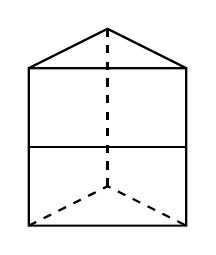
\begin{tikzpicture}
              \draw[dashed,thick] (-1,0) -- (0,0.5) edge (0,2.5) -- (1,0);
              \draw[thick] (-1,0) rectangle (1,2) -- (0,2.5) -- (-1,2);
              \draw[thick] (-1,1) -- (1,1);
            \end{tikzpicture}
            \qquad
            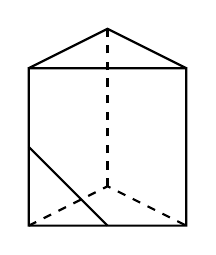
\begin{tikzpicture}
              \draw[dashed,thick] (-1,0) -- (0,0.5) edge (0,2.5) -- (1,0);
              \draw[thick] (-1,0) rectangle (1,2) -- (0,2.5) -- (-1,2);
              \draw[thick] (-1,1) -- (0,0);
            \end{tikzpicture}
          \end{center}
    \item We can take an octagon and pair up vertices:
          \begin{center}
            \tikz\graph{subgraph C_n[n=8, clockwise]; 1--5, 2--6, 3--7, 4--8};
          \end{center}
  \end{itemize}
  which, according to Wikipedia, is exhaustive.
\end{sol}

\begin{xca}
  For the subset graph $S_{n,k}$ defined in Example 4.1.5,
  find the number of vertices and the number of edges.
\end{xca}
\begin{sol}
  There are $\binom{n}{k}$ vertices.
  Each edge takes one of the $k$ elements and replaces it with a different one
  from the $n-k$ others.
  That is, each node has $k(n-k)$ edges.
  By Corollary 4.3.3, this means there are $\frac12k(n-k)\binom{n}{k}$ edges.
\end{sol}

\begin{xca}
  The \term{odd graph} $O_n$ is the graph
  whose vertices are the $n$-subsets of a $(2n+1)$-set,
  two such subsets being adjacent if and only if they are disjoint.
\end{xca}
\begin{enumerate}
  \item Draw $O_1$ and $O_2$.
        \begin{sol}
          The 1-subsets of [3] are $\{1\}$, $\{2\}$, and $\{3\}$
          where they are all disjoint.
          Then, we can draw $O_1$ (omitting curly braces) as
          \begin{center}
            \tikz\graph[clockwise]{ subgraph K_n[n=3] };
          \end{center}
          This is isomorphic to $K_3$.
          The 2-subsets of [5] are 12, 13, 14, 15, 23, 24, 25, 34, 35, and 45.
          We can draw $O_2$ as
          \begin{center}
            \tikz\graph[radius=1.6cm]{ subgraph C_n[V={12,34,15,23,14,25,13,24,35}, clockwise] -!- 45, 15--24, 35--14, 34--25, 12--45--13, 45--23 };
          \end{center}
          as desired.
        \end{sol}
  \item Prove that $O_2$ is isomorphic to the Peterson graph.
        \begin{sol}
          Observe that the layout of $O_2$ is identical to that of $H$ in Figure 4.8.
        \end{sol}
  \item How many vertices and edges does $O_n$ have?
        \begin{sol}
          There are $\binom{2n+1}{n}$ vertices.

          Each each vertex has $\binom{(2n+1)-2}{2} = \binom{2n-1}{2}$ adjacent vertices,
          giving by Corollary 4.3.3 a total of $\frac12\binom{2n+1}{n}\binom{2n-1}{2}$ edges.
        \end{sol}
\end{enumerate}

\begin{xca}
  The \term{line-graph} $L(G)$ of a graph $G$ is the graph
  whose vertex set is $E(G)$ and in which two vertices are adjacent
  if and only if the corresponding edges of $G$ are incident with a common vertex.
\end{xca}
\begin{enumerate}
  \item Find a graph $G$ such that $L(G)$ is isomorphic to $G$.
        \begin{sol}
          Let $G = K_3 = \tikz[baseline=0]\graph[radius=0.5cm,clockwise]{ subgraph K_n[n=3] };$.
          Then, $L(G) = \tikz[baseline=0]\graph[radius=0.5cm,clockwise]{ subgraph K_n[V={12,23,13}] };$
          isomorphic to $G$.
        \end{sol}
  \item Find nonisomorphic graphs $G$, $G'$ such that $L(G)$ is isomorphic to $L(G')$.
        \begin{sol}
          Let $G = K_3$ as above and
          $G' = \tikz[baseline=0]\graph[radius=0.5cm]{ subgraph K_n[clockwise, n=3] -!- 4 };$.

          Since 4 has no edges in $G'$, it does not affect $L(G')$.
          Then, $L(G) = L(G')$ (the same graph as in part (a)).
        \end{sol}
  \item If $G$ is the graph \tikz[baseline=-15pt]\graph[dots nodes]{{1,2}--3[y=-0.5]--4[y=-0.5]--{6,7}};
        find $L(G)$, $L(L(G))$ and $L(L(L(G)))$.
        \begin{sol}
          Calculate $L(G) = \tikz[baseline=-15pt]\graph[dots nodes]{{1,2}--4[y=-0.5]--{6,7}, 1--2, 6--7};$
          and $L(L(G)) = \tikz[baseline=-15pt]\graph[dots nodes]{1[y=-0.5]--{[clique] {2,3}--{4,5}}--6[y=-0.5]};$.

          Finally, $L(L(L(G))) =
            \tikz[baseline=-15pt]\graph[dots nodes, simple]{{1,2}--3[y=-0.5]--{[clique] 4[y=0.5],5[y=0.75,x=-0.35],6[y=1.25,x=0.35],7[y=1.5]}--8[y=-0.5]--{9,10}, 1--2, 9--10, 5-!-6, 4-!-7, 5--1--4, 6--2--7, 4--9--5, 6--10--7};$
        \end{sol}
\end{enumerate}

\begin{xca}
  For integer $n \geq 0$, define the graph $G_n$ as follows:
  $V(G_n)$ is the set of all binary strings of length $n$
  having at most one block of 1's.
  Two vertices are adjacent if they differ in exactly one position.
\end{xca}
\begin{enumerate}
  \item Find $\abs{V(G_n)}$.
        \begin{sol}
          We can map $V(G_n) \bijects S_{n+1,2} \cup \{\varnothing\}$ as follows:
          given $\alpha = 0^i1^j0^k \in V(G_n)$, let $f(\alpha) = \{i,j\}$.
          Then, $f^{-1}(\{\ell,m\}) = 0^\ell 1^m 0^{n-\ell-m}$.
          Map $\varnothing$ to the string $0^n$ with no 1's.
          Notice that for this to work, we define $[n+1] = \{0,\dotsc,n\}$.

          Therefore, $\abs{V(G_n)} = \binom{n+1}{2} + 1 = \frac{1}{2}n(n+1) + 1 = \frac12n^2 + \frac12n + 1$.
        \end{sol}
  \item Make drawings of $G_3$ and $G_4$.
        \begin{sol}
          Construct $V(G_3) = \{000, 100, 010, 001, 110, 011, 111\}$.
          Likewise, construct $V(G_4) = \{0000, 1000, 0100, 0010, 0001, 1100, 0110, 0011, 1110, 0111, 1111\}$.
          Then, notice that differing by exactly one position
          can either add a 1 (swap $0 \to 1$) or remove a 1 ($1 \to 0$).
          Then, we can draw
          \begin{center}
            \tikz\graph[layered layout]{ 000 --[complete bipartite] {100, 010, 001} --[complete bipartite] {110, 011} --[complete bipartite] 111 };
            \qquad
            \tikz\graph[layered layout]{ 0000 --[complete bipartite] {1000, 0100, 0010, 0001} --[complete bipartite] {1100, 0110, 0011} --[complete bipartite] {1110, 0111} --[complete bipartite] 1111 };
          \end{center}
          as desired.
        \end{sol}
  \item Find $\abs{E(G_n)}$.
        \begin{sol}
          Consider the triangle and the $0^n$ separately.
          Between each layer with $i-1$ and $i$ 0's,
          there are $i(i-1)$ edges.
          Then, $\sum_{i=2}^{n} i(i-1) = 2\sum_{i=1}^{n}\binom{i}{2} = 2\binom{n+1}{3}$.
          Finally, there are $n$ edges incident to $0^n$,
          so we have $\abs{E(G_n)} = 2\binom{n+1}{3} + n$.
        \end{sol}
\end{enumerate}

\begin{xca}\end{xca}
\begin{enumerate}
  \item Draw $K_{m,n}$ for all $m$, $n$ such that $1 \leq m \leq n \leq 3$.
        \begin{sol}
          Draw:
          \begin{center}
            \tikz\graph[dots nodes]{ subgraph K_nm[n=1,m=1] };
            \qquad
            \tikz\graph[dots nodes]{ subgraph K_nm[n=1,m=2] };
            \qquad
            \tikz\graph[dots nodes]{ subgraph K_nm[n=1,m=3] };
            \qquad
            \tikz\graph[dots nodes]{ subgraph K_nm[n=2,m=2] };
            \qquad
            \tikz\graph[dots nodes]{ subgraph K_nm[n=2,m=3] };
            \qquad
            \tikz\graph[dots nodes]{ subgraph K_nm[n=3,m=3] };
          \end{center}
          as desired.
        \end{sol}
  \item How many vertices does $K_{m,n}$ have?
        \begin{sol}
          There are $\abs{V(K_{m,n})} = m + n$ vertices.
        \end{sol}
  \item Let $K$ be a complete bipartite graph on $p$ vertices.
        Prove that $K$ has at most $\floor{p^2/4}$ edges.
        \begin{sol}
          Suppose $K \simeq K_{m,n}$.
          Then, there are $\abs{E(K)} = \abs{E(K_{m,n})} = m \times n$ edges
          to connect each of the $m$ left vertices to $n$ right vertices.

          \WLOG, suppose $m \leq n$.
          By high school algebra, $\abs{E(K)}$ is maximized when $m = n$.

          If $p$ is even, let $m = n = \frac{p}{2}$.
          Then, $\abs{E(K)} \leq \frac{p^2}{4}$.

          If $p = 2k+1$ is odd, let $m = k = \floor{\frac{p}{2}}$ and $n = k+1 = \floor{\frac{p}{2}}+1$.
          Notice that $\floor{\frac{p^2}{4}} = \frac{4k^2+4k+1}{4} = k^2+k$.
          Then, $\abs{E(K)} \leq mn = k^2 + k = \floor{\frac{p^2}{4}}$,

          Therefore, $K$ has at most $\floor{\frac{p^2}{4}}$ edges.
        \end{sol}
  \item Let $G$ be a bipartite graph on $p$ vertices.
        Prove that $G$ has at most $\floor{p^2/4}$ edges.
        \begin{sol}
          Since $G$ is bipartite, all edges cross the bipartition
          $(A,B)$ where $\abs{A} = m$ and $\abs{B} = n$.
          That is, all edges exist in $K_{m,n}$.

          Thus, $G$ is a subgraph of $K_{m,n}$
          and by (c), $\abs{E(G)} \leq \abs{E(K_{m,n})} \leq \floor{\frac{p^2}{4}}$, as desired.
        \end{sol}
  \item Let $G$ be a $k$-regular bipartite graph with bipartition $(X,Y)$.
        Prove that $\abs{X} = \abs{Y}$ if $k > 0$.
        Is this still valid when $k=0$?
        \begin{prf}
          Let $k \geq 1$ and suppose $\abs{X} \neq \abs{Y}$.

          Then, notice that since $G$ is bipartite, by definition,
          the edges incident to $X$ are the edges incident to $Y$,
          i.e., $\abs{\delta(X)} = \abs{\delta(Y)}$.
          But each of $X$ (resp.\ $Y$) consist of $\abs{X}$
          vertices of $k$ degree going to vertices in $Y$,
          so $\abs{\delta(X)} = k\abs{X} = k\abs{Y} = \abs{\delta(Y)}$.

          But $\abs{X} \neq \abs{Y}$, implying $k = 0$. Contradiction.

          This is not valid when $k=0$.
          Notice that if $V(G) = \{1\}$, $E(G) = \varnothing$,
          $X = \{1\}$, and $Y = \varnothing$,
          we have a 0-regular bipartite graph with bipartition $(X,Y)$
          and $\abs{X} \neq \abs{Y}$.
        \end{prf}
\end{enumerate}

\begin{xca}
  The \term{complement} of a graph $G$, denoted $\bar G$,
  is the graph with $V(\bar G) = V(G)$
  and the edge $uv \in E(\bar G)$ if and only if $uv \not\in E(G)$.
\end{xca}
\begin{enumerate}
  \item Let $G$ have vertices 1, 2, 3, 4 and edges 12, 23, 34, 14. Draw $\bar G$.
        \begin{sol}
          Note that $E(\bar G) = \{13,24\}$ (with $E(G)$ in dashes):
          \begin{center}
            \tikz\graph[simple necklace layout]{1,2,3,4; 1--3; 2--4; {[edges=dashed] 1--2--3--4--1, 3--4}};
          \end{center}
          as desired.
        \end{sol}
  \item Find a 5-vertex graph that is isomorphic to its complement.
        \begin{sol}
          Consider the 5-cycle $C_5$ and its complement (dashed) $\bar C_5$:
          \begin{center}
            \tikz\graph{subgraph C_n[n=5, clockwise]; {[edges=dashed] 1--3--5--2--4--1}};
          \end{center}
          and notice that the complement is the cycle $\{1,3,5,2,4\}$.
        \end{sol}
  \item Prove that no 6-vertex graph is isomorphic to its complement.
        \begin{prf}
          Notice that for a graph $G$, we have $E(G) \cup E(\bar G)$
          is a disjoint union of the set of subsets of $V(G)$ with size 2.

          Notice that for a 6-vertex graph, there are $\binom{6}{2} = 15$
          subsets of $V(G)$ with size 2.
          These cannot be partitioned into $\abs{E(G)} = \abs{E(\bar G)}$
          because 15 is odd.
        \end{prf}
  \item Let $G_1$ and $G_2$ be two graphs.
        Prove that $G_1$ is isomorphic to $G_2$
        if and only if $\bar G_1$ is isomorphic to $\bar G_2$.
        \begin{prf}
          Suppose $G_1 \simeq G_2$.
          Then, there exists an isomorphism $\phi : V(G_1) \to V(G_2)$
          such that $uv \in E(G_1) \iff \phi(u)\phi(v) \in E(G_2)$.
          It follows that
          \[ uv \in E(\bar G_1) \iff uv \not\in E(G_1) \iff \phi(u)\phi(v) \not\in E(G_2) \iff \phi(u)\phi(v) \in E(\bar G_2) \]
          so $\phi$ is also an isomorphism between $\bar G_1$ and $\bar G_2$.

          Finally, since $\bar{\bar G} = G$ (because $E(G)$ and $E(\bar G)$ are set complements),
          this goes in both directions.
        \end{prf}
  \item Find all 2-regular non-isomorphic graphs on 6 vertices
        (prove that these are the only ones).
        \begin{prf}
          Notice that a 2-regular component is a cycle.
          The smallest cycle is the 3-cycle,
          so we can either have two 3-cycles or one 6-cycle.
        \end{prf}
  \item Prove that there are only two 3-regular non-isomorphic graphs on 6 vertices.
        \begin{prf}
          Let $G$ be such a graph.
          For each vertex, there are three incident edges.
          The other two potential edges lie in the complement.
          Therefore, $\bar G$ is a 2-regular graph on 6 vertices.
          By (d), the complement preserves isomorphism.
          By (e), there are only two classes of 2-regular isomorphic graphs on 6 vertices.
          Therefore, there must be only two 3-regular non-isomorphic graphs on 6 vertices.
        \end{prf}
\end{enumerate}

\begin{xca}
  Make drawings of the 15 non-isomorphic graphs having six vertices and six edges,
  such that every vertex has degree at least one.
\end{xca}

\begin{xca}
  Are the graphs in Figure 4.14 isomorphic? Justify your answer.
\end{xca}

\begin{xca}\label{xca:prime}
  For $n$ a positive integer, define the \term{prime graph} $B_n$
  to be the graph with vertex set $\{1,2,\dotsc,n\}$,
  where $\{u,v\}$ is an edge if and only if $u + v$ is a prime number.
  Prove that $B_n$ is bipartite.
\end{xca}
\begin{prf}
  Notice that for $u+v > 2$ to be prime, it must be odd
  (since we cannot have a $\{1,1\}$ loop to make 2).
  Therefore, exactly one of $u$ and $v$ must be odd.
  It follows that if we partition $V(B_n) = [n]$
  into $X = \{ i \in [n] : i \bmod 2 = 0 \}$ and $Y = \{ i \in [n] : i \bmod 2 = 1 \}$,
  we have a bipartition of $B_n$.
\end{prf}

\subsection{How to Specify a Graph}

Not covered in Fall 2022 offering.

\subsection{Paths and Cycles}
\begin{xca}\label{xca:deg-path}
  Let $G$ be a graph with minimum degree $k$, where $k \geq 2$.
  Prove that:
\end{xca}
\begin{enumerate}
  \item $G$ contains a path of length at least $k$
        \begin{prf}
          Proceed by induction on $k$.
          Let $v \in V(G)$ be a vertex.

          If $k = 0$, then notice that $v$ is a path of length 0.

          If $k = 1$, then $v$ must have a neighbour $u$.
          Then, $v,u$ is a path of length 1.

          For $k \geq 2$, since $k > k-1$, suppose
          there exists a path $P = v_0,\dotsc,v_{k-1}$ of length $k-1$.
          Since $v_{k-1}$ has degree at least $k$, $\abs{N_G(v_{k-1})} \geq k$,
          so $\abs{N_G(v_{k-1}) \setminus \{v_0,\dotsc,v_{k-2}\}} \geq 1$.
          Let $v_k \in N_G(v_{k-1}) \setminus \{v_0,\dotsc,v_{k-2}\}$
          and notice that $P + v_k$ is a path of length $k$.
        \end{prf}
  \item $G$ contains a cycle of length at least $k+1$
        \begin{prf}
          By part (a), a path of length at least $k$ exists in $G$.
          Let $P = v_0,\dotsc,v_k,\dotsc,v_\ell$ be the longest such path.
          Then, as above, notice that $\abs{N_G(v_\ell) \setminus \{v_{\ell-k},\dotsc,v_{\ell-1}\}} \geq 1$.
          Select any $x \in N_G(v_\ell) \setminus \{v_{\ell-k+1},\dotsc,v_{\ell-1}\}$.
          If $x \not\in P$, then $P' = P + x$ is a longer path.
          Otherwise, $x = v_i$ for $0 \leq i \leq \ell-k$.

          The cycle $v_i,\dotsc,v_\ell$ has length at least $k+1$.
        \end{prf}
\end{enumerate}

\setcounter{xca}{3} % Skip adjacency matrix questions

\begin{xca}
  Let $G$ be the graph whose set of vertices is the set of all
  ``lower 48'' states of the United States, plus Washington, DC,
  with two vertices being adjacent if they share a boundary.
  Let $H$ be the subgraph of $G$ whose vertices are those of $G$
  whose first letter is one of W, O, M, A, N,
  and whose edges are the edges of G whose ends have this property.
  Find a path in $H$ from Washington to Washington, DC.
\end{xca}
\begin{sol}
  Consult a map and get WA, OR, NV, AZ, NM, OK, MO, NB, WY, MT, ND, MN, WI, MI, OH, WV, MD, DC.
\end{sol}

\begin{xca}
  Consider the word graph $W_n$ defined in Example 4.1.2.\footnote{
    $V(W_n)$ is the set of English words of length $n$
    with adjacency if they differ by exactly one letter.}
\end{xca}
\begin{enumerate}
  \item Find a cycle through \emph{math} in $W_4$.
        \begin{sol}
          (\emph{math}, \emph{meth}, \emph{mete}, \emph{mate}, \emph{math})
          is a cycle in $W_4$.
        \end{sol}
  \item Find a path from \emph{pink} to \emph{blue} in $W_4$.
        \begin{sol}
          (\emph{pink}, \emph{tink}, \emph{tank}, \emph{tans}, \emph{tens}, \emph{fens}, \emph{feus}, \emph{flus}, \emph{flue}, \emph{blue})
          using words in Merriam--Webster.
        \end{sol}
\end{enumerate}

\begin{xca}
  For $n \geq 2$, prove that the $n$-cube contains a Hamilton cycle.
\end{xca}
\begin{prf}
  Let $G_n$ denote the $n$-cube. Proceed by induction on $n$.

  Notice that for $n = 2$, $(00,01,11,10,00)$ is a Hamilton cycle.

  Let $n \geq 3$.
  Partition $V(n) = V_0 \cup V_1$ based on the first digit in the binary string.
  Now, the subgraphs induced by $V_0$ and $V_1$ are isomorphic to $G_{n-1}$
  under the isomorphism $f_b : G_{n-1} \to V_b : \alpha \mapsto b\alpha$
  and inverse $f^{-1}_b : V_b \to G_{n-1} : b_1\cdots b_n \to b_2 \cdots b_n$.

  Assume $G_{n-1}$ has a Hamilton cycle.
  \WLOG, suppose that it begins at $0^{n-1}$ and ends at $0^{n-2}1$,
  so that $V_0$ has a Hamilton cycle $(00^{n-2}0, \dotsc, 00^{n-2}1)$
  and $V_1$ has a Hamilton cycle $(10^{n-2}0, \dotsc, 10^{n-2}1)$.

  Then, $(00^{n-2}0, \dotsc, 00^{n-2}0, 10^{n-2}0, \dotsc, 10^{n-2}1, 00^{n-2}1)$
  is a Hamilton cycle for $G_n$.
\end{prf}

\begin{xca}
  Prove that the complete bipartite graph $K_{m,n}$ has a Hamilton cycle
  if and only if $m = n$ and $m > 1$.
\end{xca}
\begin{prf}
  Suppose $m = n$ and $m > 1$.
  Then, $(s_1,t_1,s_2,t_2,\dotsc,s_m,t_n)$ is a Hamilton cycle.

  Conversely, assume \Wlog that $m \leq n$ and that there is a Hamilton cycle.

  When $m = 0$, there are no edges and no Hamilton cycle.
  For $m = 1$, trace the Hamilton cycle starting at $s_1$.
  First $N(s_1) = \{t_i\}$, so the next vertex must be $t_k$ for some $k$.
  However, $N(t_k) = \{s_1\}$ and we cannot continue because $s_1t_k$ is already in the cycle.

  Otherwise, suppose $m \neq n$ and $1 < m < n$.
  Every edge is $s_i t_j$, so the cycle goes $s_{a_1},t_{b_1},s_{a_2},t_{b_2},\dotsc$.
  At $t_{b_m}$, we have visited $m$ vertices $s_i$, i.e., all of them.
  Therefore, the cycle must end here and return to $s_{a_1}$.
  However, there are vertices $t_{b_{m+1}},\dotsc,t_{b_n}$ which are not in the cycle.
  That is, the cycle is not a Hamilton cycle.

  Therefore, there is a Hamilton cycle if and only if $m = n$ and $m > 1$.
\end{prf}

\begin{xca}\label{xca:oddcycle}
  Show that if there is a closed walk of odd length in the graph $G$,
  then $G$ contains an odd cycle
  (that is, $G$ has a subgraph which is a cycle on an odd number of vertices).
\end{xca}
\begin{prf}
  Suppose that $W = v_1,\dotsc,v_n,v_1$
  is the shortest closed walk of odd length that exists in $G$ (i.e., $n$ is odd).

  Induct on the number of such vertices in $W$ that appear multiple times.

  If $W$ is a path, i.e., there are no such vertices, $W$ is a cycle and we are done.

  Otherwise, there exists $i$ and $j$ such that $v_i = v_j$.
  Then, the edges in $W$ can be partitioned into two closed walks
  $W_1 = v_1,\dotsc,v_{i-1},v_i,v_{j+1},\dotsc,v_1$ and $W_2 = v_i,v_{i+1},\dotsc,v_{j-1},v_i$.
  Since $W$ has an odd number of edges and $E(W_1) \cup E(W_2)$ partition $E(W)$,
  exactly one of $W_1$ and $W_2$ has an odd number of edges.
  By the inductive hypothesis, since that walk necessarily has fewer duplicates,
  there exists an odd cycle in that walk.

  Therefore, there exists an odd cycle in $G$.
\end{prf}

\begin{xca}
  A \term{diagonal} of a cycle in a graph is an edge that joins vertices
  that are not consecutive in the cycle.
\end{xca}
\begin{enumerate}
  \item Prove that a shortest cycle has no diagonal.
        \begin{prf}
          Let $C = v_1,\dotsc,v_k,v_1$ be a shortest cycle.
          Suppose a diagonal $v_iv_j$, $i < j$, $j \neq i + 1$ exists.
          Then, $v_1,\dotsc,v_i,v_j,\dotsc,v_k,v_1$
          is a shorter cycle. Contradiction.
        \end{prf}
  \item Prove that a shortest odd cycle has no diagonal.
        \begin{prf}
          Let $C = v_1,\dotsc,v_k,v_1$ be a shortest odd cycle, i.e., $k$ is odd.
          Suppose a diagonal $v_iv_j$, $i < j$, $j \neq i + 1$ exists.
          Then, as in \cref{xca:oddcycle}, we can create two cycles
          $C_1 = v_1,\dotsc,v_i,v_j,\dotsc,v_k,v_1$
          and $C_2 = v_i,\dotsc,v_j,v_i$.

          Since $V(C_1) \cap V(C_2) = \{v_i,v_j\}$,
          we have $\abs{V(C)} = \abs{V(C_1)} + \abs{V(C_2)} - 2$.
          That is, $1 \equiv \abs{V(C_1)} + \abs{V(C_2)} \pmod{2}$.
          Then, either $C_1$ or $C_2$ must be a shorter odd cycle.
          Contradiction.
        \end{prf}
  \item Give an example of a graph in which a shortest even cycle has a diagonal.
        \begin{sol}
          The minimal example \tikz[baseline=-3pt]\graph[dots nodes, radius=0.5cm]{ subgraph C_n[n=4, clockwise], 1--3 };.
        \end{sol}
\end{enumerate}

\begin{xca}\end{xca}
\begin{enumerate}
  \item Prove that a $k$-regular graph of girth 4 has at least $2k$ vertices ($k \geq 2$).
  \item For $k = 2,3$, find a $k$-regular graph of girth 4 with precisely $2k$ vertices.
        Generalize these examples to find one for each $k \geq 2$.
  \item Prove that a $k$-regular graph of girth 5 has at least $k^2+1$ vertices ($k \geq 2$).
  \item Prove that a $k$-regular graph of girth $2t$, where $t \geq 2$,
        has at least $\frac{2(k-1)^t-2}{k-2}$ vertices.
  \item Prove that a $k$-regular graph of girth $2t+1$, where $t \geq 2$,
        has at least $\frac{k(k-1)^t-2}{k-2}$ vertices.
  \item For $k = 2,3$, give an example of a $k$-regular graph of girth 5
        with exactly $k^2+1$ vertices.
\end{enumerate}

\setcounter{subsection}{9}
\subsection{Equivalence Relations, Connectedness, Eulerian Circuits, Bridges}

\begin{xca}
  Prove that the prime graph $B_n$ defined in \Cref{xca:prime} is connected for every $n$.
  You may use without proof the following fact:
  For every integer $k \geq 2$,
  there is a prime number $r$ such that $k < r < 2k$.
\end{xca}
\begin{prf}
  Proceed by induction on $n$.
  Clearly, $B_1$ is connected with a single vertex.

  Let $n \geq 2$. We may assume that $B_{n-1} = B_n - n$ is connected.

  There exists a prime number $r$ such that $n < r < 2n$.
  That is, $r = n + m$ for $1 \leq m \leq n-1$.
  Since $m \in \{1,\dotsc,n-1\} \subseteq [n] = V(B_n)$,
  the edge $mn$ exists in $B_n$.
  For any $k \in V(B_n) \setminus \{n\} = V(B_{n-1})$,
  since $B_{n-1}$ is connected, there exists a $k,m$-path.
  Adjoining $mn$, there exists a $k,n$-path in $B_n$.

  Therefore, by Theorem 4.8.2, $B_n$ is connected.
\end{prf}

\begin{xca}
  Prove that if $G$ is connected,
  any two longest paths have a vertex in common.
\end{xca}
\begin{prf}
  Let $P_1$ be a $s,t$-path and $P_2$ be a $u,v$-path in $G$
  such that both $P_1$ and $P_2$ are longest paths in $G$ with length $k$.

  Then, suppose that $V(P_1) \cap V(P_2) = \varnothing$.

  Since $G$ is connected, there exists a $t,u$-path $P_3$ in $G$.
  Consider the walk $W = P_1P_3P_2$.
  By the process in the proof in Theorem 4.6.2,
  there exists a $s,v$-path $P$ using all the non-overlapping
  vertices in $P_1$ and $P_2$ (but only some of $P_3$).
  That is, $P$ has length at least $2k$, meaning that $P_1$ and $P_2$ are not longest paths.

  Therefore, by contradiction, $P_1$ and $P_2$ must share a vertex.
\end{prf}

\begin{xca}
  Which graphs, with at least one edge,
  have the property that every edge is a bridge?
\end{xca}
\begin{sol}
  By Theorem 4.10.3, an edge is a bridge if and only if it is not contained in a cycle.
  Therefore, every edge is a bridge if and only if the graph contains no cycles.
  That is, the graph is a forest.
\end{sol}

\begin{xca}
  If every vertex of a graph $H$ with $p$ vertices has degree at least $\frac{p}{5}$,
  prove that $H$ cannot have more than 4 components.
\end{xca}
\begin{prf}
  Let $v \in V(H)$. Since $\deg v \geq \frac{p}{5}$,
  its component has size at least $\frac{p}{5} + 1$.

  This applies to all components, so if there are $k$ components,
  $p \geq k(\frac{p}{5}+1)$, that is, $k \leq \frac{p}{\frac{p}{5}+1} < \frac{p}{p/5} = 5$.
  Therefore, there are at most 4 components.
\end{prf}

\begin{xca}
  If an edge $e$ is not a bridge of a connected graph $G$,
  prove that $e$ is an edge of some cycle.
\end{xca}
\begin{prf}
  If $e = uv \in E(G)$ is not a bridge, then $G - e$ remains connected.
  But that means there is a $u,v$-path $P$ in $G - e$.
  Then, $P + e$ is a cycle in $G$ containing $e$.
\end{prf}

\begin{xca}
  Prove that a 4-regular graph has no bridge.
\end{xca}
\begin{prf}
  Consider an edge $e = uv$ in a 4-regular component $G$.
  Then, by the proof of \Cref{xca:deg-path}, $e$ lies in a 5-cycle.
  Since $e$ lies in a cycle, it is not a bridge by Theorem 4.10.3.
\end{prf}

\begin{xca}\label{xca:4107}
  Let $A_n$ be the graph whose vertices are the $\{0,1\}$-strings of length $n \geq 2$,
  and edges are between strings that differ in exactly two positions.
\end{xca}
\begin{enumerate}
  \item How many edges does $A_n$ have?
        \begin{sol}
          Since each of the $2^n$ strings have $\binom{n}{2}$ neighbours
          (must pick two positions to change),
          we have $\abs{E(A_n)} = \binom{n}{2}2^{n-1}$ by the Handshaking Lemma.
        \end{sol}
  \item Is $A_n$ bipartite for any $n \geq 2$?
        \begin{sol}
          When $n = 2$, $V(A_2) = \{00,01,10,11\}$
          and $E(A_2) = \{\{00,11\},\{01,10\}\}$
          which is bipartite with bipartition $(X,Y) = (\{00,11\},\{01,10\})$.

          For $n \geq 3$, there exists an odd cycle
          $(0000^{n-3}, 0110^{n-3}, 1100^{n-3}, 0000^{n-3})$.
          Therefore, by Theorem 5.3.2, $A_n$ is not bipartite.
        \end{sol}
  \item How many components does $A_n$ have?
        \begin{sol}
          Claim: there are two components.

          Divide the elements of $V(A_n)$ by parity.
          Notice that changing exactly two positions either sends
          two 0's to two 1's, two 1's to two 0's, or one of each (cancelling).
          These do not change the parity.
          Therefore, no path exists between any string of even and odd parity.

          Now, consider two strings with the same parity.
          Then, they differ by an even number of positions.
          By changing two at a time, there exists a path between them.

          Therefore, there are exactly two components of $A_n$.
        \end{sol}
\end{enumerate}

\begin{xca}
  Let $B_n$ be the graph whose vertices are the $\{0,1\}$-strings of length $n \geq 2$,
  and edges are between strings that differ in exactly two consecutive positions.
\end{xca}
\begin{enumerate}
  \item How many edges does $B_n$ have?
        \begin{sol}
          The neighbours of a string can differ in the positions starting at $1,\dotsc,n-1$.
          That is, the degree of every vertex is $n-1$.
          By the Handshaking Lemma, since $\abs{V(B_n)} = 2^n$,
          $\abs{E(B_n)} = (n-1)2^{n-1}$.
        \end{sol}
  \item How many components does $B_n$ have?
        \begin{sol}
          There are at least two components by \Cref{xca:4107}.

          Consider two strings with even parity.
          Follow a path sending each instance of 01 to 10.
          This will give a string of the form $1^{2k}0^{n-2k}$.
          Then, there is clearly a path to $0^n$.
          Therefore, all the even parity strings form a single component by Theorem 4.8.2.

          Likewise, for odd parity strings, there is always a path to $10^{n-1}$
          and they form a single component by Theorem 4.8.2.

          Therefore, there are exactly two components of $B_n$.
        \end{sol}
\end{enumerate}

\begin{xca}
  Let $G$ be a graph in which exactly two of the vertices $u$ and $v$ have odd degree.
  Prove that $G$ contains a path from $u$ to $v$.
\end{xca}
\begin{prf}
  Suppose there is not a $u,v$-path.
  That is, $u$ and $v$ lie in different components.
  Then, every $w \in [u]$, $w \neq u$ has even degree.
  By the Handshaking Lemma, 
  \[ 
    0 \equiv 2\abs{E(G)}
    \equiv \sum_{w \in [u]} \deg(w)
    \equiv \deg(v) + \sum_{\substack{w \in [u] \\ w \neq v}}\deg(w)
    \equiv 1 + \sum_{\substack{w \in [u]\\w \neq v}}0 \equiv 1 \pmod{2}
  \]
  which is a contradiction. Therefore, $v \in [u]$ and there must exist a $u,v$-path.
\end{prf}

\section{Trees}

\subsection{Trees}

\begin{xca}
  \begin{enumerate}
    \item Draw one tree from each isomorphism class of trees on six or fewer vertices.
    \item For each tree in (a), exhibit a bipartition $(X,Y)$ by coloring the vertices
          in $X$ with one colour and the vertices in $Y$ with another.
  \end{enumerate}
\end{xca}
\begin{sol}
  Draw the trees:
  \begin{center}
    \tikz\graph[dots tree]{6[red]--1[blue]--{2[red]--3[blue], 4[red]--5[blue]}}; \qquad
    \tikz\graph[dots tree]{1[red]--{2[blue]--3[red], 4[blue]--5[red]--6[blue]}}; \qquad
    \tikz\graph[dots tree]{3[red]--{1[blue]--2[red], 4[blue]--{5[red],6[red]}}}; \qquad
    \tikz\graph[dots tree]{1[red]--{2[blue]--{3[red],4[red]}, 5[blue], 6[blue]}}; \qquad
    \tikz\graph[dots tree]{2[red]--{1[blue], 3[blue]--{4[red],5[red],6[red]}}}; \qquad
    \tikz\graph[dots tree]{1[red]--{2[blue],3[blue],4[blue],5[blue],6[blue]}}; \qquad
  \end{center}
  where we colour the vertices an even distance away from the root
  in \textcolor{red}{red} and those an odd distance away in \textcolor{blue}{blue}.
\end{sol}

\begin{xca}
  Prove that every tree is bipartite.
\end{xca}
\begin{prf}
  Let $T$ be a non-empty tree and $r \in V(T)$.

  Then, by Lemma 5.1.3, for all vertices $u \in V(T)$,
  there exists a unique path $P_u$ from $u$ to $r$.
  Define $P_r = \varnothing$.
  Claim that $X = \{ u \in V(T) : \text{length of $P_u$ even} \}$
  and $Y = \{ u \in V(T) : \text{length of $P_u$ odd} \}$
  are a bipartition of $T$.

  Let $uv \in E(T)$.
  Then, either $P_v = P_u + uv$ or $P_u = P_v + uv$
  because if $uv$ is in both paths, then there exists a cycle
  based on the walk $(r,P_u,u,v,P_v,r)$.
  \WLOG, suppose $P_v = P_u + uv$.
  Then, the length of $P_v$ is exactly one more than the length of $P_u$.
  That is, the parity is different.
  Therefore, $u$ and $v$ are partitioned by $(X,Y)$.

  It follows that $T$ is bipartite.
\end{prf}

\begin{xca}\label{xca:leaf-from-deg}
  What is the smallest number of vertices of degree 1 in a tree
  with 3 vertices of degree 4 and 2 vertices of degree 5?
  Justify your answer by proving that this is the smallest possible number
  and by giving a tree with this many vertices of degree 1.
\end{xca}
\begin{sol}
  Let $n_r$ be the number of vertices with degree $r$ in such a tree.
  By the alternate proof of Theorem 5.1.8,
  $n_1 = 2 + \sum_{r \geq 3}(n-2)n_r = 2 + n_3 + 2n_4 + 3n_5 + \sum_{r \geq 6}(n-2)n_r$.
  If $n_4 = 3$ and $n_5 = 2$, then $n_1 \geq 2 + 6 + 6 = 14$.

  Construct the tree:
  \begin{center}
    \begin{tikzpicture}
      \graph[dots nodes, layered layout, grow down, sibling distance=0.5cm] {
        4a--{4b--{a,b,c},4c--{e,f,g},5a--{i,j,k,l},5b--{n,o,p,q}}
        };
    \end{tikzpicture}
  \end{center}
  which has 14 leaves.
\end{sol}

\begin{xca}
  Find the smallest number $r$ of vertices in a tree having
  two vertices of degree 3, one vertex of degree 4, and two vertices of degree 6.
  Justify your answer by proving that any such tree has at least $r$ vertices,
  and by giving an example of such a tree with exactly $r$ vertices.
\end{xca}
\begin{sol}
  As in \cref{xca:leaf-from-deg}, write $n_1 = 2 + n_3 + 2n_4 + 3n_5 + 4n_6 + \sum_{r \geq 7}(n-2)n_r$
  and notice that if $n_3 = 2$, $n_4 = 1$, and $n_6 = 2$,
  then $n_1 \geq 2 + 2 + 2 + 8 = 14$.
  Draw the tree:
  \begin{center}
    \begin{tikzpicture}
      \graph[dots nodes, layered layout, grow down, sibling distance=0.5cm] {
        4a--{3a--{1,2},3b--{4,5},6a--{6,7,8,9,10},6b--{11,12,13,14,15}}
        };
    \end{tikzpicture}
  \end{center}
  which has 14 leaves.
\end{sol}

\begin{xca}
  A cubic tree is a tree whose vertices have degree either 3 or 1.
  Prove that a cubic tree with exactly $k$ vertices of degree 1
  has $2(k - 1)$ vertices.
\end{xca}
\begin{prf}
  As in \cref{xca:leaf-from-deg}, $k =: n_1 = 2 + n_3$ so $n_3 = k - 2$.
  Then, there are $n_1 + n_3 = k + k - 2 = 2(k-1)$ vertices in total.
\end{prf}

\begin{xca}
  Prove that a forest with $p$ vertices and $q$ edges has $p - q$ components.
\end{xca}
\begin{prf}
  Let $G$ be such a forest and $T_1,\dotsc,T_k$ be its $k$ components,
  which are all trees because they are connected and have no cycles.
  By Theorem 5.1.5, $\abs{E(T_i)} = \abs{V(T_i)} - 1$, so
  \[
    q = E(G) = \sum_{i=1}^k \abs{E(T_i)}
    = \sum_{i=1}^k  (\abs{V(T_i) - 1})
    = \qty(\sum_{i=1}^k \abs{V(T_i)}) - k
    = p - k
  \]
  so $k = p - q$, as desired.
\end{prf}

\begin{xca}
  Let $p \geq 2$. Show that a sequence of $(d_1,\dotsc,d_p)$ of positive integers
  is the degree sequence of a tree on $p$ vertices if and only if
  $\sum_{i=1}^p d_i = 2p-2$.
\end{xca}
\begin{prf}
  Suppose that $T$ is a tree with $V(T) = \{v_1,\dotsc,v_p\}$.
  Let $d_i = \deg(v_i)$. Then, apply Theorem 5.1.5 ($\abs{E(T)} = p-1$)
  and the Handshaking Lemma ($\sum d_i = 2\abs{E(T)} = 2p - 2$), as desired.

  Suppose that $\delta = (d_1,\dotsc,d_p)$ is a sequence with sum $2p-2$.
  We induct on $p$.

  If $p=2$, then $2p-2 = 2$.
  There is only one composition of 2, $\delta = (1,1)$.
  Draw the tree \tikz\graph[dots tree]{1--2}; with two vertices of degree 1.

  Let $p \geq 3$.
  Since all the $p$ parts of the sequence are positive, i.e., $d_i \geq 1$,
  we have $\sum d_i \geq p$.
  Then, by the pigeonhole principle, since there remains $p-2$ weight to distribute
  into $p$ parts of the sequence, there exists $d_i = 1$ and $d_j > 1$ for distinct $i,j$.
  Let $\delta'$ be $\delta$ with $d_j \mapsto d_j-1$ and skipping $d_i$.
  This is a sequence of $p-1$ elements that sums to $(2p-2)-2 = 2(p-1)-2$.

  Inductively, a tree $T'$ of $p-1$ vertices exists with degree sequence $\delta'$.
  Then, add a leaf to $v_j \in V(T)$, i.e., a vertex of degree 1,
  and increase the degree of $v_j$ by 1.
  This is a tree of $p$ vertices with degree sequence $\delta$.

  Therefore, by induction, $\delta$ is the degree sequence of a tree of $p$ vertices.
\end{prf}

\setcounter{subsection}{2}
\subsection{Spanning Trees, Characterizing Bipartite Graphs}

\begin{xca}
  Let $r$ be a fixed vertex of a tree $T$.
  For each vertex $v$ of $T$, let $d(v)$ be
  the length of the path from $v$ to $r$ in $T$. Prove that
\end{xca}
\begin{enumerate}
  \item for each edge $uv$ of $T$, $d(u) \neq d(v)$, and
        \begin{prf}
          Let $P_u$ and $P_v$ be the paths from $u$ and $v$ to $r$, respectively.

          Suppose $uv \not\in P_u$ and $uv \not\in P_v$.
          Then, $(u,P_u,r,P_v,v)$ is a $(u,v)$-walk in $T-uv$,
          meaning a $(u,v)$-path exists in $T-uv$.
          But then $T$ has two $(u,v)$-paths because $(u,uv,v)$ is a path,
          contradicting Lemma 5.1.3.
          Therefore, $uv \in P_u$ or $uv \in P_v$.

          \WLOG, suppose $uv \in P_u$.
          That is, $P_u = (u,uv,v,\dotsc,r) = u + P_v$
          because $P_v$ is the unique path from $v$ to $r$ in $T$.
          Therefore, $d(u) = \abs{E(P_u)} \neq \abs{E(P_v)} + 1 = d(v)$.
        \end{prf}
  \item for each vertex $x$ of $T$ other than $r$,
        there exists a unique vertex $y$
        such that $y$ is adjacent to $x$ and $d(y) < d(x)$.
        \begin{prf}
          Let $P_x = (x,y,\dotsc,r)$ be the unique $(x,r)$-path (note that $y$ could be $r$).
          Clearly, $\delta(y) < \delta(x)$ since the unique $(y,r)$-path
          is contained inside $P_x$.

          Let $z \in N_T(x)$, $z \neq y$.
          Suppose $P_z$ does not contain $P_x$.
          Then, $(z,P_z,r,P_x,x,xz,z)$ is a cycle in $T$.
          By contradiction, $P_z$ contains $P_x$ and $d(z) > d(x)$.

          Therefore, $y$ is unique.
        \end{prf}
\end{enumerate}

\subsection{Breadth-First Search}

Not covered in Fall 2022 offering.

\subsection{Applications of Breadth-First Search}

Not covered in Fall 2022 offering.


\section{Codes}

Not covered in Fall 2022 offering.

\section{Planar Graphs}

\setcounter{subsection}{2}
\subsection{Planarity, Euler's Formula, Stereographic Projection}

\begin{xca}
  Prove that every planar embedding has either a vertex of degree at most 3
  or a face of degree 3.
\end{xca}
\begin{prf}
  Let $G$ be a component of a planar graph.

  If $G$ has no faces (besides the outer face),
  then $G$ is a tree with at least two leaves (by Theorem 5.1.8)
  and those leaves have degree $1 \leq 3$.

  Otherwise, let $V = \abs{V(G)}$,
  $E = \abs{E(G)}$, and $F = \abs{F(G)}$.
  Then, by Euler's Formula, $V - E + F = 2$.

  Suppose that all vertices have degrees at least 4
  and all faces have degrees at least 4.
  Then, by the Handshaking Lemma, $2E = \sum \deg(v) \geq 4V$ so $E \geq 2V$.
  Likewise, by the Faceshaking Lemma, $2E = \sum \deg(f) \geq 4F$ so $E \geq 2F$.
  That is, $2E \geq 2(V + F)$, i.e., $E \geq V + F$.
  But then $2 = (V + F) - E < 0$, a contradiction.

  Therefore, there either exists a vertex with degree at most 3
  or a face of degree 3.\footnote{Note that inner faces have degree at least 3
    and smaller degree implies a tree.}
\end{prf}

\begin{xca}
  Prove that each of the graphs shown in Figure 7.6 is planar,
  by exhibiting a planar embedding.
\end{xca}
\begin{sol}
  Draw planar embeddings:
  \begin{tikzpicture}
    \graph{subgraph C_n[V={b,c,d,i,e,f,g}, clockwise] -!- h, {b,c,i,e,f,g}--h, a[y=1.2,x=2]--{c,d}, a--[bend right]b, a--[bend left]i, f--[out=130,in=90,looseness=1.2]a};
  \end{tikzpicture}
  \quad
  \begin{tikzpicture}
    \graph{subgraph C_n[V={c,g,b,f,a,i,e,h}, clockwise], f--{e,c,g}, d[x=-2], d--{h,i}, a--[bend left]d, c--[bend right]d, f--[out=-100,in=-90,looseness=1.3]d};
  \end{tikzpicture}
\end{sol}

\begin{xca}
  Let $n \geq 3$ be an integer.
  Suppose that a convex $n$-gon is drawn in the plane
  and then each pair of nonadjacent corner points
  is joined by a straight line through the interior.
  Suppose that no three of these lines through the interior
  meet at a common point in the interior.

  Let $f_n$ be the number of regions into which
  the interior of the $n$-gon is divided by this process.
  Use Euler's Formula to find $f_n$.
\end{xca}
\begin{sol}
  Let $v_n$, $e_n$, and $f_n$ be the number of vertices, edges, and faces as described.
  Picking four corners of the $n$-gon uniquely determines
  a pair of intersecting lines (i.e., an added vertex),
  so we have in total $v_n = n + \binom{n}{4}$ vertices.

  Each vertex from the $n$-gon has degree $n-1$
  and each new vertex has degree 4 (as the intersection of two lines),
  so by the Handshaking Lemma, $2e = n(n-1) + 4\binom{n}{4}$
  or equivalently $e = \binom{n}{2} + 2\binom{n}{4}$.

  Therefore, by Euler's Formula, discounting the outer face because
  we are counting only the interior of the $n$-gon, $f_n = 1 - v_n + e_n
    = 1 - n + \binom{n}{2} + \binom{n}{4}$.\footnote{This is a \href{https://www.youtube.com/watch?v=K8P8uFahAgc}{3Blue1Brown} video.}
\end{sol}

\subsection{Platonic Solids}

Not covered in Fall 2022 offering.

\setcounter{subsection}{5}
\subsection{Nonplanar Graphs, Kuratowski's Theorem}

\setcounter{subsection}{7}
\subsection{Colouring and Planar Graphs, Dual Planar Maps}

\section{Matchings}

\setcounter{subsection}{1}
\subsection{Matchings, Covers}

\subsection{K\"onig's Theorem}

\setcounter{subsection}{5}
\subsection{Applications of K\"onig's Theorem, Systems of Distinct Representatives, Perfect Matchings in Bipartite Graphs}

\setcounter{subsection}{7}
\subsection{Edge-Colouring, Application to Timetabling}

Not covered in Fall 2022 offering.


\end{document}
